\documentclass[a4paper, oneside]{discothesis}

\usepackage[utf8]{inputenc}
\usepackage[T1]{fontenc}
\usepackage{CJKutf8}
\usepackage{tikz}
\usepackage{graphicx}
\usepackage{subcaption}
\usetikzlibrary{calc,shapes,arrows,positioning}


%%%%%%%%%%%%%%%%%%%%%%%%%%%%%%%%%%%%%%%%%%%%%%%%%%%%%%%%%%%%%%%%%%%%%%%%%%%%%%%%%%%%%%%%%%%%%%%%%
% DOCUMENT METADATA

\thesistype{Towards more data-driven, and less biased decisions in startup investing with AI workflows} % Master's Thesis, Bachelor's Thesis, Semester Thesis, Group Project
\title{Moon AI: automating VC}

\author{Angelo Giacco}
\email{agiacco@ethz.ch}

\institute{ETH AI Centre \\[2pt]
ETH Zürich}

\logo{\includegraphics[width=0.2\columnwidth]{figures/eth_ai_center.png}}

\supervisors{Isabelle Siegrist\\[2pt] Prof. Dr. Elliott Ash}

% Optionally, keywords and categories of the work can be shown (on the Abstract page)
%\keywords{Keywords go here.}
%\categories{ACM categories go here.}

\date{\today}

%%%%%%%%%%%%%%%%%%%%%%%%%%%%%%%%%%%%%%%%%%%%%%%%%%%%%%%%%%%%%%%%%%%%%%%%%%%%%%%%%%%%%%%%%%%%%%%%%

\begin{document}

\frontmatter % do not remove this line
\maketitle

\cleardoublepage

\begin{acknowledgements}
	I would like to express my sincere gratitude to several individuals who have been instrumental in the completion of this thesis. First and foremost, I extend my heartfelt thanks to my advisor, Isabelle Siegrist, for her invaluable guidance, and to Professor Elliott Ash for his mentorship. It was only by pure chance that we collaborated, but I am very grateful that we did.

A big thanks to everyone at Beugi that made my year in Switzerland so wonderful and full of hike/ski days.

I owe as always a special debt of gratitude to my family for their love and support.

    \begin{CJK*}{UTF8}{gbsn}
最后,我要特别感谢我的伴侣萧庭恩。她始终如一的支持和对我的信任是我前进的动力。\clearpage\end{CJK*}
\end{acknowledgements}



\begin{abstract}
    The venture capital (VC) industry has in recent years experienced a significant shift towards a solo General Partner (GP) model, where a single partner, often a successful former founder or early hire at a unicorn, raises a fund to invest in upcoming entrepreneurs. Solo-GPs are more agile but lack the platform services and in depth analysis available to VC firms with large teams. Simultaneously, Large Langauge Models (LLMs) have emerged as powerful multi-task learners. This has led to the emergence of AI-copilots powered by LLMs for multi-task reasoning emerging in various verticals. 
    
    This thesis explores the creation of a new product: MoonAI. MoonAI is a venture investing copilot designed to empower solo GPs and traditional VC firms alike, by providing a copilot capable of emulating a team of analysts. By employing large language models for reasoning, structured output to guide agents, and matryoshka embeddings to semantically search the internet, the system extracts relevant signals for startup investing from vast amounts of unstructured data publicly available on the internet. The end result is a tool that helps assist in sourcing startups and generating investment memos.
    
    MoonAI can be customised to align with various investment hypotheses, supporting solo GPs in their sourcing and due diligence processes and removing the need for duplicate platform teams at each VC firm. In the future, we aim for MoonAI to evolve into a comprehensive data science and investing platform.
    
    By creating this adaptable infrastructure, MoonAI seeks to democratise access to high-quality investment platforms, encourage data-driven investing, and thereby democratise access to capital. The project's core thesis posits that successful VC firms and especially solo-GPs will increasingly rely on automated research analysts to identify, analyse and support upcoming entrepreneurs, with MoonAI positioning itself at the forefront of this transformation.
    
    This thesis provides an overview of the advances in Natural Language Processing that make MoonAI possible, an overview of the VC industry, and details how the product was built. 
\end{abstract}


\begin{zusammenfassung}
Die Venture-Capital-Branche (VC) hat in den letzten Jahren eine bedeutende Verlagerung hin zu einem Modell mit einem einzelnen General Partner (GP) erlebt, bei dem erfolgreiche ehemalige Gründer aufstrebende Unternehmer unterstützen.
Gleichzeitig haben sich Large Language Models (LLMs) als leistungsfähige Multi-Task-Lerner etabliert. Dies hat dazu geführt, dass in verschiedenen Bereichen KI-Copiloten entstanden sind, die sich auf LLMs für Multi-Task-Reasoning stützen.
CopyDiese Arbeit untersucht die Entwicklung eines neuen Produkts, MoonAI, eines innovativen Venture-Investing-Copiloten, der sowohl einzelne GPs als auch traditionelle VC-Firmen unterstützen soll, indem er als Copilot fungiert, der ein Team von Analysten emulieren kann.
Durch den Einsatz von Large Language Models für Reasoning, strukturierte Ausgaben zur Steuerung von Agenten und Matryoshka-Embedding für semantische Internetsuchen extrahiert das System relevante Signale für Startup-Investitionen aus großen Mengen unstrukturierter Internetdaten.

Derzeit als Memo-Generierungstool mit einem einfachen CRM-Layout verpackt, strebt MoonAI an, sich zu einer umfassenden Plattform für Data Science und Investitionen zu entwickeln. Das System kann an verschiedene Investitionshypothesen angepasst werden, um einzelne GPs bei ihren Sourcing- und Due-Diligence-Prozessen zu unterstützen und die Notwendigkeit von doppelten Plattform-Teams in jeder VC-Firma zu eliminieren.

Durch die Schaffung dieser anpassungsfähigen Infrastruktur zielt MoonAI darauf ab, den Zugang zu hochwertigen Investitionsplattformen zu demokratisieren, datengetriebenes Investieren zu fördern und dadurch den Zugang zu Kapital zu demokratisieren. Die Kernthese des Projekts postuliert, dass erfolgreiche VC-Firmen und insbesondere einzelne GPs zunehmend auf automatisierte Research-Analysten zurückgreifen werden, um aufstrebende Unternehmer zu unterstützen, wobei sich MoonAI an der Spitze dieser Transformation positioniert.

Diese Arbeit bietet einen Überblick über die Fortschritte in der Natürlichen Sprachverarbeitung, die MoonAI ermöglichen, einen Überblick über die VC-Branche und detaillierte Informationen darüber, wie das Produkt entwickelt wurde.
\end{zusammenfassung}

\tableofcontents

\mainmatter % do not remove this line

% Start writing here
\chapter{Introduction}

The venture capital (VC) industry stands at the forefront of innovation, playing a crucial role
in identifying and nurturing startups that have the potential to disrupt industries and drive
economic growth. Indeed, Acs et al. ~\cite{acs} find that startups are key catalysts for economic growth, 
not only creating new markets but also stimulate competition and innovation in existing ones, bringing economic dynamism across multiple sectors. 

The VC industry invests in startups with significant potential to disrupt industries and drive economic growth. 
VC investments returns follow a power law distribution, with a long tail of successful investments. 
A study of 21,000 financings from 2004-2013 by Correlation Ventures found that 65\% of financings fail to return 1x capital ~\cite{levine2014venture}, 
thus the remaining 35\% must return significantly more to generate a net-return that is acceptable. 
VCs rely on a small number of portfolio investments to achieve outstanding paybacks: enough to cover for losses and
still produce substantial profits. To generate these substantial outcomes, startups rely on the external funding from VCs
to achieve rapid growth, often depicted by a "hockey stick" growth curve ~\cite{marmer}.

The power law nature of startups means that the competition to get on the best deals is incredibly intense, and those 
deals are also the only ones that matter. The top 2\% of VC funds capture 95\% of industry
returns ~\cite{bai}. Particularly at the earliest stage of the investment lifecycle (pre- Series A), there is a scarcity of
reliable information ~\cite{dellermann}. As a result, VCs often rely heavily on human judgment which is prone to bias. 
This may yield sub-optimal decisions ~\cite{cummingdai} and could explain why women-led startups only received 2.1\% of all venture capital invested in 2023 ~\cite{pitchbook2024vc}.
Traditionally, VC firms have relied heavily on human intuition, personal networks, and experience
to identify promising investment opportunities. While this approach has yielded success, it is
not without limitations. Human decision-making is susceptible to biases, inconsistencies, and the
constraints of processing vast amounts of information.

VCs have increasingly adopted data-driven investing practices to combat these biases. 
Traditional gradient boosting approaches have been used successfully, and in recent years the growth of data volume has ushered deep learning (DL) into the industy ~\cite{eqt}.
For example, graph neural networks have been used to predict a startup's success based on its links to a wider startup ecosystem ~\cite{korea}. 
These models can integrate diverse data sources, including structured information about startups, founders, and investors ~\cite{corea}, as well as unstructured data from social networks and web sources. 
Preliminary findings suggest that data-driven VCs may be more likely to back founders from underrepresented backgrounds, potentially addressing systemic biases in the industry ~\cite{futureVC}.

In recent years, the VC landscape has experienced a shift towards the practice solo General Partners (GPs)  raising funds, meanwhile fund raising has been increasingly strained for non-elite VC firms since the end of zero interest rates. Unlike traditional VC firms, with rigid investment deal processes, solo GPs can make investment decisions quickly and independently, which is particularly valuable in competitive deal environments where rapid decision-making can be crucial.
In contrast, the formation of new traditional VC firms has slowed in recent years. This can be attributed to several factors, including the trend towards larger fund sizes, which makes it challenging for new firms to compete and gain traction with the returns from the VC industry becoming concentrated among well-established firms that enjoy significant advantages in deal flow and fundraising. 
The difficulty for smaller VCs to raise funds means they will have less resources for research, contributing to their worse performance.

Solo GPs and smaller funds have extremely limited resources which may amplify the issues of bias and incomplete information in the investment process, forcing them to  focus on a narrower pool of potential investments, potentially overlooking promising opportunities outside their immediate network (Huang et al., 2020). Furthermore, without the resources to explore a wide range of sectors or geographies, solo GPs might gravitate towards familiar industries or founder profiles, potentially limiting the diversity of their investment portfolios (Gompers et al., 2021) and limiting opportunities for under represented founders. In addition, the agility of solo GPs will intensify the competition and rush to produce term sheets for 'hot' startups. 

In response to these challenges, a project at the ETH AI Center of ETH Zurich aims to introduce automation to VC firms and facilitate the adoption of data-driven investing practices. 
The project focuses on developing an AI-powered tool for generating investment memoranda. This approach aims to streamline the decision-making process for investment analysts, significantly reducing the time spent on screening potential investments. 
Utilising multimodal data and state-of-the-art language models, the system aggregates diverse data sources, including pitch decks, financial data, and web information, to provide a comprehensive analysis of investment opportunities.
Furthermore, this project introduces tools for data-driven investing that aim to reduce bias in the investment process by incorporating objective insights, broadening investment scope, identifying overlooked startups, informing decisions with diverse data points, and standardising evaluation processes. Developing the MoonAI product is the first phase of this project; subsequent research will analyse its ability to reduced bias decision making. 

The potential impact of such a tool is multifaceted. First, it addresses the resource disparity
between solo GPs/smaller VC firms and larger VC firms, potentially democratising access to high-quality investment
analysis. Second, it introduces a data-driven approach to complement human intuition in the
investment process, potentially reducing biases and improving decision-making accuracy
~\cite{dellermann}. Finally, by streamlining the sourcing and evaluation processes, MoonAI
could allow VCs to consider a broader range of startups by reducing the cognitive load of analysing a startup, potentially leading to a more diverse
and inclusive investment landscape (Brush et al., 2019).

While the VC industry has been facing challenges, Large Language Models (LLMs) have emerged as powerful tools capable of multi-task reasoning and processing vast amounts of
unstructured data (Brown et al., 2020) and transformed the field of Natural Language Processing (NLP). These advancements have led to the development of
AI-powered copilots in various industries, augmenting human capabilities and decision-making processes.
 Large Language Models (LLMs) are particularly well-suited to be a venture capital copilot and decision-making support for several key reasons. 
Firstly, LLMs excel at pattern matching, a crucial skill in the venture capital industry. They can analyze vast amounts of unstructured data from various sources, 
identifying trends, similarities, and potential success indicators that might not be immediately apparent to human analysts.
They can rapidly process and synthesize information from a wide range of publicly available sources, including news articles, social media, academic publications, 
and industry reports. This ability enables a comprehensive understanding of a startup's market position, competitive landscape, and potential growth trajectory 
without relying solely on information provided by the startup itself.
Furthermore, LLMs offer simple yet powerful workflow automation capabilities. They can streamline many time-consuming aspects of the venture capital process, 
such as initial startup screening, report generation, and even preliminary financial analysis. By automating these routine tasks, LLMs free up valuable time 
for venture capitalists to focus on higher-level strategic decisions and relationship building with promising founders. This efficiency gain is particularly 
beneficial for solo GPs or smaller VC firms with limited resources, allowing them to compete more effectively with larger, more established firms.
The combination of these capabilities makes LLMs an ideal tool for augmenting human decision-making in venture capital. They can provide data-driven insights,
 reduce information asymmetry, and increase the overall efficiency of the investment process. 
 
 As the venture capital landscape continues to evolve and 
 become more competitive, the integration of LLMs into investment workflows has the potential to significantly enhance the accuracy, speed, and scope of investment decisions, ultimately leading to better outcomes for both investors and entrepreneurs.

This thesis explores the intersection of these trends through the development of MoonAI, an
AI-powered venture investing copilot designed to empower both solo GPs and traditional VC firms.
By leveraging state-of-the-art LLMs, structured output for guided reasoning, advanced
semantic search capabilities, and agentic workflows, MoonAI aims to speed up the startup evaluation process and remove repetitive tasks from a VC. The
system is designed to extract relevant signals for startup investing from the vast pool of
publicly available unstructured data on the internet, assisting in sourcing startups and
generating comprehensive investment memos. By addressing these questions and developing a practical tool for the VC industry, this thesis
aims to contribute to the ongoing dialogue about the role of AI in financial decision-making and
its potential to reshape the startup ecosystem. The following chapters will explore the
technical foundations of Large Language Models, provide a review of the Venture Capital industry, and give an overview and evaluation of the MoonAI platform. 

\chapter{Natural Language Processing}

In this section, the recent in advances in Natural Language Processing will be discussed. First, we will consider the basics of machine learning, 
then consider the standard approaches to NLP used in the past prior to the emergence of deep learning and discuss the advances that have been made in recent years that have enabled large language models to become state of the art at virtually all tasks in the field of NLP.

Many of these advances have been possible due to the parallelizability of training thanks to the Transformer architecture which make use of advances in GPUs. How GPUs are able to parallelize the training of large language models is beyond the scope of this overview, but it is important to note that this is a significant advance that has revolutionised the field of NLP. It can be summarised as follows: GPUs have significantly accelerated the training of transformer-based models by leveraging their ability to perform massive parallel computations, which make them ideal for matrix multiplications, the operation underpinning the self-attention mechanism in transformers and the feed-forward layers. 
GPUs excel at these tasks due to their architecture, which is designed to handle many simple calculations simultaneously.
This GPU-driven acceleration has been a key factor in enabling the training of increasingly large and complex language models, pushing the boundaries of what's possible in NLP.

Before we consider the essentials of machine learning that enable the training of large language models, let us first specify the objective of a large language model more clearly. 
This will also motivate the use of the Transformer architecture, and clarify why other methods, from n-gram based approaches to other flavours of DL like recurrent neural networks, are not suited for the task.

\begin{theorem}[Language Modelling Objective] \label{thm:first theorem}
    Given an alphabet $\Sigma$ and a distinguished end-of-sequence symbol $\texttt{eos} \notin \Sigma$, a
    language model is a collection of conditional probability distributions $p(y \mid w)$ for $y \in \Sigma \cup \{\texttt{eos}\}$ and $w \in \Sigma^*$,
    the Kleene closure of $\Sigma$.
\end{theorem}

We therefore can obtain the probability of a string according to a particular language model by autoregressively factorising:

\begin{equation}
    P(w) = P(w_1, \ldots, w_n) =  P(\texttt{EOS} \mid w) \cdot \prod_{i=1}^n P(w_i \mid w_1, \ldots, w_{i-1}) 
\end{equation}

With the objective of crafting a model able to learn this function p in mind, let us begin our exploration of machine learning. 

\section{Modelling Data}

This thesis assumes familiarity with the basics of machine learning. Nevertheless, a brief summary is provided here to establish a foundation.

In classical computer programming, humans define a set of explicit rules and provide input data. The computer then processes new data according to the defined rules to produce an output for the data. This approach works well for problems with clear, unchanging rules and predictable inputs ~\cite{russell2010artificial}.

Machine learning, on the other hand, inverts this paradigm: rules are learnt by applying processing to data. It can be broadly categorised into two main types: supervised and unsupervised learning ~\cite{murphy2012machine}.

In supervised learning, humans provide a large dataset of input-output pairs (often referred to as training data). 
The machine learning algorithm then attempts to learn the underlying patterns or rules that map the inputs to the outputs ~\cite{hastie2009elements}. 
This learned model can then be used to make predictions or decisions on new, unseen data.
Supervised learning is particularly useful for tasks such as classification and regression ~\cite{bishop2006pattern}.

In unsupervised learning, the algorithm is given input data without corresponding output labels. The goal is to discover hidden patterns or structures within the data ~\cite{ghahramani2004unsupervised}. Common unsupervised learning tasks include clustering, dimensionality reduction, and anomaly detection ~\cite{hinton2006reducing}.

The key advantage of machine learning is its ability to handle complex, non-linear relationships in data and to adapt to new patterns without being explicitly reprogrammed ~\cite{goodfellow2016deep}. 
This makes it particularly useful for tasks like natural language processing, where the rules governing language use are clearly too complex and nuanced to be explicitly coded ~\cite{jurafsky2009speech}.

\subsection{Losses}
To begin our search for a model that best describes the underlying patterns in our data, it is necessary to have a way of describing how accurate our model's predictions are. This is done by defining a loss function that measures the difference between the model's predictions and the ground-truth values ~\cite{goodfellow2016deep}.

In the context of natural language processing where we typically have the option of predicting multiple labels for a single input, an evident choice for the loss function is cross-entropy, which has its basis in information theory as a measure of the difference between two probability distributions ~\cite{shannon1948mathematical}.

The cross-entropy loss, denoted as $H(p,q)$, for a classification task with $C$ classes is defined as:

\begin{equation}
    H(p,q) = -\sum_{i=1}^C p(i) \log q(i)
\end{equation}

where $p(i)$ is the true probability distribution (usually a one-hot encoded vector for the true class) and $q(i)$ is the predicted probability distribution from the model ~\cite{murphy2012machine}.

For binary classification, this simplifies to:

\begin{equation}
    H(p,q) = -[y \log(\hat{y}) + (1-y) \log(1-\hat{y})]
\end{equation}

where $y$ is the true label (0 or 1) and $\hat{y}$ is the predicted probability of the positive class ~\cite{bishop2006pattern}.

In the context of language modeling, where we're predicting the next token in a sequence, the cross-entropy loss is calculated over the entire vocabulary at each step:

\begin{equation}
    L = -\sum_{t=1}^T \sum_{v=1}^V y_{t,v} \log(\hat{y}_{t,v})
\end{equation}

where $T$ is the sequence length, $V$ is the vocabulary size, $y_{t,v}$ is 1 if token $v$ is the true next token at position $t$ and 0 otherwise, and $\hat{y}_{t,v}$ is the model's predicted probability for token $v$ at position $t$ ~\cite{jurafsky2009speech}.

Minimising this loss encourages the model to assign higher probabilities to the correct next tokens in the training data, thus learning the underlying patterns of the language ~\cite{bengio2003neural}.

Given some neural network architecture $\mathcal{A}$, a parameter space $\Theta \subset \mathbb{R}^d$ is induced, where $d$ is the total number of parameters in the network. Each point $\theta \in \Theta$ represents a specific configuration of the network's parameters ~\cite{lecun2015deep}.

Let $\mathcal{L}: \Theta \rightarrow \mathbb{R}$ be the loss function that measures the performance of the model on the given task. The goal of training the neural network can then be formally expressed as an optimization problem:

\begin{equation}
    \theta^* = \arg\min_{\theta \in \Theta} \mathcal{L}(\theta)
\end{equation}

where $\theta^*$ represents the optimal set of parameters that minimizes the loss function over the entire parameter space $\Theta$. This optimization problem encapsulates the essence of training a neural network: finding the configuration of parameters that yields the best performance according to the chosen loss function ~\cite{rumelhart1986learning}.


\subsection{Optimising Parameters}

\subsubsection{Gradient Descent}

Gradient descent is a fundamental optimization algorithm used in training neural networks. It iteratively adjusts the model parameters in the direction of steepest descent of the loss function. The basic update rule for gradient descent is:

\begin{equation}
    \theta_{t+1} = \theta_t - \eta \nabla \mathcal{L}(\theta_t)
\end{equation}

where $\theta_t$ are the parameters at iteration $t$, $\eta$ is the learning rate, and $\nabla \mathcal{L}(\theta_t)$ is the gradient of the loss function with respect to the parameters.

Calculating the loss over the entire batch is typically very expensive, which motivates the use of Stochastic Gradient Descent (SGD) -  where the gradient is computed using a single randomly selected training example in each iteration or Mini-batch SGD - which uses a small subset of the training data in each iteration.

\subsubsection{Automatic Differentiation}

To enable gradient descent, Automatic Differentiation (AutoDiff) libraries allow for efficient and accurate computation of gradients. AutoDiff libraries rely on the chain rule. 

Mathematically, for a composite function $f(g(x))$, the chain rule states:

\begin{equation}
    \frac{df}{dx} = \frac{df}{dg} \cdot \frac{dg}{dx}
\end{equation}

AutoDiff systems leverage this principle to compute gradients through arbitrarily complex computational graphs ~\cite{griewank2008evaluating}. Modern deep learning frameworks like PyTorch and TensorFlow have built-in AutoDiff capabilities, which greatly simplify the implementation of new models and training procedures ~\cite{paszke2019pytorch, abadi2016tensorflow}. These systems maintain a computational graph of operations and use it to automatically compute gradients, enabling efficient training of large-scale neural networks, allows researchers to focus on designing network architectures and loss functions, while the AutoDiff system handles the intricate details of gradient computation ~\cite{baydin2018automatic}.

\subsubsection{Optimisation}

Several advanced optimization algorithms have been developed to improve upon basic SGD. Momentum adds a fraction of the previous update to the current one, helping to accelerate convergence and reduce oscillations ~\cite{sutskever2013importance}:
\begin{equation}
    v_{t+1} = \gamma v_t + \eta \nabla \mathcal{L}(\theta_t)
\end{equation}
\begin{equation}
    \theta_{t+1} = \theta_t - v_{t+1}
\end{equation}
where $\gamma$ is the momentum coefficient.

RMSprop adapts the learning rate for each parameter based on the historical gradient magnitudes ~\cite{tieleman2012lecture}:
\begin{equation}
    s_{t+1} = \beta s_t + (1-\beta)(\nabla \mathcal{L}(\theta_t))^2
\end{equation}
\begin{equation}
    \theta_{t+1} = \theta_t - \frac{\eta}{\sqrt{s_{t+1} + \epsilon}} \nabla \mathcal{L}(\theta_t)
\end{equation}
where $\beta$ is the decay rate and $\epsilon$ is a small constant for numerical stability.

The most widely adopted optimizer in practice, Adam, combines ideas from momentum and RMSprop, maintaining both a running average of gradients and their squared values ~\cite{kingma2014adam}:
\begin{equation}
    m_{t+1} = \beta_1 m_t + (1-\beta_1)\nabla \mathcal{L}(\theta_t)
\end{equation}
\begin{equation}
    v_{t+1} = \beta_2 v_t + (1-\beta_2)(\nabla \mathcal{L}(\theta_t))^2
\end{equation}
\begin{equation}
    \theta_{t+1} = \theta_t - \frac{\eta}{\sqrt{\hat{v}_{t+1}} + \epsilon} \hat{m}_{t+1}
\end{equation}
where $\hat{m}_{t+1}$ and $\hat{v}_{t+1}$ are bias-corrected estimates of $m_{t+1}$ and $v_{t+1}$ respectively.

These advanced optimizers often lead to faster convergence and better generalization in practice ~\cite{ruder2016overview}.

\subsubsection{Initialisation}

Proper initialization of neural network parameters is crucial for effective training. The naive approach of initialising all weights to zero is not viable, as this would cause all neurons to learn the same features. Two popular initialization methods have been developed.

Xavier Initialization, proposed by Glorot and Bengio, is designed to maintain the variance of activations and gradients across layers. For a layer with $n_{in}$ input units and $n_{out}$ output units, weights are initialised from a uniform distribution:

\begin{equation}
    W \sim U\left(-\sqrt{\frac{6}{n_{in} + n_{out}}}, \sqrt{\frac{6}{n_{in} + n_{out}}}\right)
\end{equation}

This initialization works well for layers with linear activations or tanh activations, helping to prevent the vanishing or exploding gradient problem in deep networks.

He Initialization, proposed by He et al., is particularly suited for layers with ReLU activations. In this method, weights are initialised from a normal distribution:

\begin{equation}
    W \sim N\left(0, \sqrt{\frac{2}{n_{in}}}\right)
\end{equation}

This approach helps maintain the variance of the outputs, which is especially important for deep networks with ReLU activations, as it prevents vanishing or exploding gradients.

Both Xavier and He initialization methods aim to set initial parameters that neither shrink nor amplify the input signal excessively. By doing so, they facilitate smoother optimization and faster convergence during the training process, ultimately leading to more effective and efficient neural network models \cite{glorot2010understanding, he2015delving}.

\subsubsection{Normalisation}

Normalisation techniques play a crucial role in neural network training and are used in the dominant Transformer architecture. Two prominent approaches, Batch Normalisation and Layer Normalisation, have been developed to address challenges related to internal covariate shift and to stabilize the distribution of layer inputs throughout the training process.

Batch Normalisation, introduced by Ioffe and Szegedy \cite{ioffe2015batch}, normalizes the inputs of each layer for each mini-batch:
\begin{equation}
    \hat{x} = \frac{x - \mu_B}{\sqrt{\sigma_B^2 + \epsilon}}
\end{equation}
where $\mu_B$ and $\sigma_B^2$ are the mean and variance of the mini-batch, and $\epsilon$ is a small constant for numerical stability. Batch Normalisation helps reduce internal covariate shift, allows higher learning rates, and acts as a regularizer.

Layer Normalisation, proposed by Ba et al. \cite{ba2016layer}, normalizes the inputs across the features:
\begin{equation}
    \hat{x} = \frac{x - \mu}{\sqrt{\sigma^2 + \epsilon}}
\end{equation}
where $\mu$ and $\sigma^2$ are the mean and variance computed over all features for each data point.

Both Batch Normalisation and Layer Normalisation help stabilize the distribution of layer inputs throughout training, mitigating the vanishing/exploding gradient problem and enabling more efficient training of deep neural networks \cite{santurkar2018does}. These techniques maintain appropriate scaling of activations and gradients throughout the network during the entire training process.

\subsection{Regularisation}

Regularisation techniques are employed to prevent overfitting and improve the generalisation of neural networks \cite{goodfellow2016deep}. Overfitting occurs when a model learns the training data too well, and thereby learns also its noise and peculiarities, leading to poor performance on unseen data. This can happen because the model becomes too complex and starts to memorize the training examples rather than learning general patterns. Regularisation methods aim to strike a balance between fitting the training data and maintaining performance on unseen data \cite{bishop2006pattern}.

Dropout, for example, randomly "drops out" a proportion of neurons during training, forcing the network to learn more robust features \cite{srivastava2014dropout}. During inference, all neurons are used but their outputs are scaled:

\begin{equation}
    y = f(Wx) \odot m, \quad m_i \sim \text{Bernoulli}(p)
\end{equation}

where $p$ is the probability of keeping a neuron active.

Early Stopping monitors the validation error during training and stops when it starts to increase, preventing the model from overfitting to the training data \cite{prechelt1998early}.

Weight Decay adds a penalty term to the loss function based on the L2 norm of the weights \cite{krogh1992simple}:

\begin{equation}
    \mathcal{L}_{new}(\theta) = \mathcal{L}(\theta) + \lambda \|\theta\|_2^2
\end{equation}

where $\lambda$ is the weight decay coefficient. This encourages smaller weights and simpler models.

These regularisation techniques, often used in combination, help in training more robust models that perform well on unseen data \cite{kukavcka2017regularization}.

\section{Historical Language Representations}

Natural Language Processing (NLP) has evolved significantly over the years, with various techniques developed to represent and analyze textual data. This section explores the historical approaches to language representation that laid the foundation for modern NLP methods. We will discuss three key techniques that were widely used before the advent of deep neural networks: N-grams, Word Document Frequency, and Topic Modelling. These methods played crucial roles in tasks such as text classification, information retrieval, and document analysis, and their principles continue to influence contemporary NLP approaches \cite{manning1999foundations}.

\subsection{N-grams}
N-grams are contiguous sequences of n items from a given sample of text or speech. In the context of natural language processing, these items are typically words or characters. N-grams have been a fundamental technique in language modeling and various NLP tasks for several decades \cite{jurafsky2000speech}.

The concept of n-grams was introduced in the early days of computational linguistics. One of the seminal papers that popularised the use of n-grams in language modeling is "A Mathematical Theory of Communication" by Claude Shannon (1948), which laid the foundation for information theory and introduced the idea of using probabilistic models for language \cite{shannon1948mathematical}.

N-grams achieved state-of-the-art performance in many NLP tasks throughout the 1990s and 2000s. For instance, the paper "An Empirical Study of Smoothing Techniques for Language Modeling" by Chen and Goodman (1996) demonstrated the effectiveness of various n-gram models for language modeling tasks \cite{chen1996empirical}. Another influential work, "A Bit of Progress in Language Modeling" by Goodman (2001), showed how n-gram models could be extended and improved for better performance \cite{goodman2001bit}.

Google Translate, one of the most widely used machine translation systems, initially relied heavily on n-gram models. Specifically, it used a 5-gram language model, as described in the paper "Large Language Models in Machine Translation" by Brants et al. (2007). This approach allowed Google Translate to capture local context and produce more fluent translations compared to earlier rule-based systems \cite{brants2007large}.

However, despite their historical success, n-grams have limitations that make them sub-optimal for modern language models. One significant limitation is their restricted context, as n-grams can only capture local context within a fixed window size. This constraint makes it challenging to model long-range dependencies in language, which are crucial for understanding complex sentences and maintaining coherence across paragraphs \cite{bengio2003neural}. Another issue is sparsity; as n increases, the number of possible n-grams grows exponentially, leading to data sparsity issues. This makes it difficult to estimate probabilities for rare or unseen n-grams accurately \cite{katz1987estimation}. N-gram models also lack semantic understanding, treating words as discrete symbols without considering their meaning or relationships. This limitation hinders their ability to capture semantic similarities between words or phrases \cite{mikolov2013distributed}. Additionally, traditional n-gram models operate on a fixed vocabulary, making it difficult to handle out-of-vocabulary words or adapt to new domains \cite{jelinek1980interpolated}. Lastly, the memory requirements for n-gram models can be substantial, as storing probabilities for all possible n-grams can be memory-intensive, especially for large values of n \cite{heafield2011kenlm}.

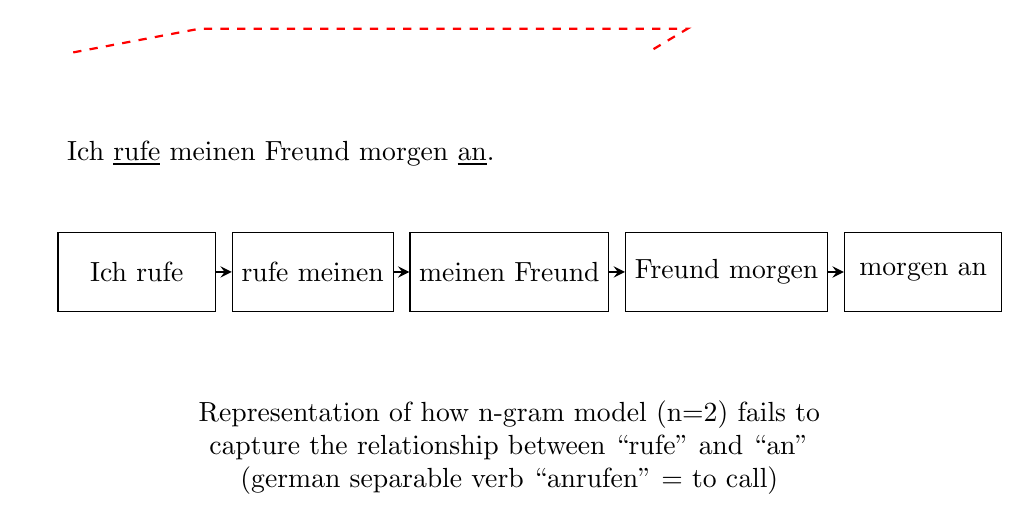
\begin{tikzpicture}[
    box/.style={draw, rectangle, minimum width=2cm, minimum height=1cm},
    arrow/.style={->, >=stealth, thick},
    node distance=0.5cm
]

% The sentence
\node[anchor=west] (sentence) at (0,0) {Ich \underline{rufe} meinen Freund morgen \underline{an}.};

% N-gram boxes
\node[box, below=1cm of sentence.west, anchor=north west] (box1) {Ich rufe};
\node[box, right=0.2cm of box1] (box2) {rufe meinen};
\node[box, right=0.2cm of box2] (box3) {meinen Freund};
\node[box, right=0.2cm of box3] (box4) {Freund morgen};
\node[box, right=0.2cm of box4] (box5) {morgen an};

% Arrows
\foreach \i in {1,...,4}
    \draw[arrow] (box\i) -- (box\the\numexpr\i+1);

% Explanation
\node[text width=12cm, below=1cm of box3, align=center] (explanation) {
    Representation of how n-gram model (n=2) fails to capture the relationship between ``rufe'' and ``an''\\
    (german separable verb ``anrufen'' = to call)
};

% Highlighting the issue
\draw[red, thick, dashed] ($(sentence.north west)+(0.2cm,1)$) -- ++(1.6cm,0.3cm) -- ++(6.2cm,0) -- ++(-0.5cm,-0.3cm);

\end{tikzpicture}

These limitations have led to the development of more advanced techniques, such as neural network-based language models and transformer architectures, which can capture longer-range dependencies, understand semantic relationships, and generate more coherent and contextually appropriate text.

\subsection{Document Term Matrices}
Document Term Matrices (DTMs) are a fundamental representation in natural language processing and information retrieval. They provide a structured way to represent a collection of documents as a matrix, where each row corresponds to a document and each column represents a unique term in the corpus.

In a basic DTM, each cell contains the frequency of a term in a particular document. 
However, this simple frequency count can be refined using more sophisticated weighting schemes, such as Term Frequency-Inverse Document Frequency (TF-IDF).

\subsubsection{TF-IDF Weighting}
TF-IDF is a statistical measure used to evaluate the importance of a word in a document relative to a collection of documents. It is calculated as the product of two components:

\begin{equation}
\text{TF-IDF}(t,d,D) = \text{TF}(t,d) \cdot \text{IDF}(t,D)
\end{equation}

Where:
\begin{equation}
\text{TF}(t,d) = \frac{\text{frequency of term t in document d}}{\text{total number of terms in document d}}
\end{equation}

\begin{equation}
\text{IDF}(t,D) = \log\left(\frac{\text{total number of documents in corpus D}}{\text{number of documents containing term t}}\right)
\end{equation}

TF-IDF weighting helps to reduce the impact of common words that appear frequently across many documents while emphasising terms that are rare and specific to certain kinds of documents.

\subsubsection{Cosine Similarity}
Cosine similarity is a metric used to measure the similarity between two non-zero vectors in a multi-dimensional space. In the context of DTMs, it is often used to compare documents or queries. The cosine similarity between two documents is calculated as the cosine of the angle between their vector representations in the term space.

Mathematically, for two document vectors A and B, the cosine similarity is given by:

\begin{equation}
\text{cosine similarity} = \frac{A \cdot B}{\|A\| \|B\|}
\end{equation}

Where $A \cdot B$ is the dot product of the vectors, and $\|A\|$ and $\|B\|$ are their Euclidean norms. We will revisit the the cosine similarity in the context of word embeddings. 

A notable example of their application in natural language processing is the work by Burgess et al. in their paper "Legislative Influence Detectors: Identifying Influential Actors in the Legislative Process" \cite{burgess2016legislative}. In this study, the authors used DTMs and cosine similarity to analyze the influence of various actors on legislative outcomes.
The researchers constructed DTMs from legislative texts and stakeholder submissions, then used cosine similarity to measure the textual similarity between final legislation and the various inputs. This allowed them to quantify the influence of different stakeholders on the legislative process, providing valuable insights into policy-making dynamics.

While Document Term Matrices (DTMs) have been widely used in natural language processing, they have significant limitations. Bengio et al. \cite{bengio2003neural} highlighted that traditional n-gram models and DTM-based approaches suffer from the curse of dimensionality and fail to capture semantic similarities between words.
The curse of dimensionality refers to the exponential increase in possible word sequences as sequence length grows, leading to data sparsity and generalization difficulties. For example, with a 10,000-word vocabulary, there are 10,000 possible one-word sequences, but $10^{20}$ possible five-word sequences.
As vocabulary size grows, the number of dimensions increases, potentially leading to overfitting on smaller datasets and processing difficulties with large corpora. Moreover, DTMs fail to capture semantic relationships between words, treating each word as a distinct dimension regardless of meaning. 
This means semantically similar words like "car" and "automobile" are represented as entirely different dimensions.

\subsection{Topic Modelling}
Topic modelling is a statistical method for discovering abstract topics that occur in a collection of documents. The most popular and widely used technique is Latent Dirichlet Allocation.

\subsubsection{Latent Dirichlet Allocation (LDA)}
Latent Dirichlet Allocation, introduced by Blei, Ng, and Jordan in 2003 \cite{blei2003latent}, is a generative probabilistic model for collections of discrete data such as text corpora. 
LDA models documents are mixtures of topics, and topics probability distribution over words.

The mathematical formula of LDA can be expressed as follows:

\begin{equation}
p(\mathbf{w}, \mathbf{z}, \boldsymbol{\theta}, \boldsymbol{\phi} | \alpha, \beta) = 
\prod_{d=1}^M p(\theta_d | \alpha) 
\left( \prod_{n=1}^{N_d} p(z_{dn} | \theta_d) p(w_{dn} | z_{dn}, \boldsymbol{\phi}) \right)
\prod_{k=1}^K p(\phi_k | \beta)
\end{equation}

Where:
\begin{itemize}
    \item $\mathbf{w}$ represents the observed words
    \item $\mathbf{z}$ represents the topic assignments
    \item $\boldsymbol{\theta}$ represents the document-topic distributions
    \item $\boldsymbol{\phi}$ represents the topic-word distributions
    \item $\alpha$ and $\beta$ are hyperparameters of the Dirichlet priors
    \item $M$ is the number of documents
    \item $N_d$ is the number of words in document $d$
    \item $K$ is the number of topics
\end{itemize}

Griffiths and Steyvers \cite{griffiths2004finding} applied LDA to analyze the abstracts of papers published in Proceedings of the National Academy of Sciences (PNAS), 
extracting 300 topics from 28,154 abstracts published 1991 to 2001. The model captured the rise and fall of scientific topics over time, reflecting changing research trends.
Topic modelling techniques like LDA has been widely adopted in social sciences, providing researchers with powerful tools to explore and analyze large text collections, 
but superior alternatives based on prompting large language models have emerged ~\cite{WangPrakashPromptTopic}. LDA itself is unsuitable for language modelling  in its
ability for language modelling due to its bag-of-word assumption which hides semantic information and fixed topic assumption.  

\section{Embeddings}

To overcome the the limitations of other representations, word embeddings were developed to offer a more efficient and semantically rich representation of language. Word embeddings are dense vector representations of words in a continuous vector space, typically of much lower dimensionality than DTMs (usually 50-300 dimensions). Each word is represented by a fixed-length vector of real numbers encoding semantic and syntactic information, effectively addressing the curse of dimensionality and reducing computational complexity and storage requirements compared to sparse DTMs. By representing words in a continuous space, embeddings facilitate better generalization to unseen words or rare word combinations, addressing the sparsity problem inherent in discrete representations. Additionally, pre-trained word 
embeddings can be used as input features for various NLP tasks, enabling transfer learning and improving performance on tasks with limited training data. 

% prehistory  The approach proposed here is also related to previous proposals of character-based text compression using neural networks to predict
% the probability of the next character (Schmidhuber, 1996). The idea of using a neural network for
% language modeling has also been independently proposed by Xu and Rudnicky (2000), although
% experiments are with networks without hidden units and a single input word, which limit the model
% to essentially capturing unigram and bigram statistics

\subsection{A Neural Probabilistic Language Model}
Yoshua Bengio introduced the concept of word embeddings in 2003 \cite{bengio2003neural}, proposing a novel approach that simultaneously learned two crucial components: (1) a distributed feature vector for each word, with a dimensionality of just 30 compared to a vocabulary size of 17,000, and (2) the probability function of word sequences. 
The model consisted of a linear projection layer to obtain the low-dimensional vector, which was followed by a non-linear hidden layer and an output layer to compute the logits. The model improved perplexity by 20\% over trigram models, but Bengio noted that the embeddings did not capture polysemous words well, and that the model could be improved by using a-priori information, for example from WordNet. Polysemous words are those that have multiple meanings or senses depending on the context (e.g., "bank" can refer to a financial institution or the edge of a river). This limitation highlights the challenge of representing words with multiple meanings in a single fixed-length vector. 

\subsection{word2vec}
In 2013, Tomas Mikolov and colleagues at Google introduced word2vec, a highly efficient method for learning high-quality word embeddings \cite{mikolov2013efficient}. Word2vec significantly improved upon previous methods by dramatically reducing computational complexity while maintaining or improving the quality of the resulting word vectors.

Word2vec proposed two model architectures: Continuous Bag-of-Words (CBOW) and Skip-gram. Both models use a shallow neural network to learn word embeddings, but they differ in their objectives. 
The CBOW model predicts a target word given its context words. The context is typically a symmetric window of words around the target.
On the other hand, the skip-gram model does the opposite, predicting the context words given a target word.
\begin{figure}[h]
    \centering
    \begin{subfigure}[b]{0.45\textwidth}
        \centering
        \includegraphics[width=\textwidth]{figures/cbow.png}
        \caption{Continuous Bag-of-Words Model}
        \label{fig:cbow}
    \end{subfigure}
    \hfill
    \begin{subfigure}[b]{0.45\textwidth}
        \centering
        \includegraphics[width=\textwidth]{figures/skipgram.png}
        \caption{Skip-gram Model}
        \label{fig:skipgram}
    \end{subfigure}
    \caption{Word2Vec Model Architectures}
    \label{fig:word2vec}
\end{figure}

The vector embeddings are learned through the process of training these models. As the model tries to predict words based on their context (or vice versa), it adjusts the word vectors to maximize the probability of correct predictions. This process leads to words that appear in similar contexts having similar vector representations.

A striking feature of word2vec embeddings is their ability to capture semantic relationships between words. This is often demonstrated through vector arithmetic. For example, the canonical example is the equation "king - man + woman $\approx$ queen" which shows that the learned embeddings encode meaningful semantic and syntactic relationships, and support mathematical operations.

\begin{figure}[h]
    \centering
    \includegraphics[width=0.5\textwidth]{figures/word2vec_analogy.png}
    \caption{Embeddings support maths operations: king - man + woman $\approx$ queen}
    \label{fig:word2vec_analogy}
\end{figure}

Word2vec became a cornerstone of many NLP applications and paved the way for further advancements in word embedding techniques.

\subsection{GloVe}
Global Vectors for Word Representation (GloVe), introduced by Pennington et al. \cite{pennington2014glove}, is a popular word embedding method that aims to capture the meaning of words by analyzing how frequently they co-occur with other words in a large corpus.

GloVe combines two approaches to create word embeddings. The first approach is global matrix factorization, which looks at the overall statistics of word co-occurrences in the entire corpus. The second approach is local context window methods, which considers the immediate context around each word. By integrating these two methods, GloVe aims to capture both the global and local aspects of word relationships in its embeddings.

The key insight behind GloVe is that the ratio of co-occurrence probabilities of two words can reveal aspects of their meaning. For example, the fact that "ice" co-occurs more frequently with "solid" than with "gas" tells us something about the nature of ice.

GloVe learns word vectors by optimising the following objective function:

\begin{equation}
J = \sum_{i,j=1}^V f(X_{ij})(\mathbf{w}_i^T\tilde{\mathbf{w}}_j + b_i + \tilde{b}_j - \log X_{ij})^2
\end{equation}

Where:
\begin{itemize}
    \item $V$ is the size of the vocabulary
    \item $X_{ij}$ is the number of times word $j$ occurs in the context of word $i$
    \item $\mathbf{w}_i$ and $\tilde{\mathbf{w}}_j$ are word vectors
    \item $b_i$ and $\tilde{b}_j$ are scalar biases
    \item $f(X_{ij})$ is a weighting function
\end{itemize}

By minimising this function, GloVe learns word vectors that capture meaningful semantic relationships between words. When it was introduced, GloVe demonstrated performance comparable to word2vec on various NLP tasks, while providing a more interpretable model of how it captures word meanings.

\subsection{ELMo}
ELMo (Embeddings from Language Models), introduced by Peters et al. in 2018 \cite{peters2018deep}, marked a significant advancement in word embedding techniques. Unlike its predecessors, ELMo produces dynamic, contextualised word embeddings that capture complex characteristics of word use, including syntax and semantics, and how these uses vary across linguistic contexts.

The key innovation of ELMo lies in its use of a deep, bidirectional LSTM model trained on a large text corpus. This model consists of a character-level convolutional neural network (CNN) that captures subword information and a two-layer bidirectional LSTM that processes the output of the CNN
ELMo generates word embeddings by taking a weighted sum of the internal states of this LSTM. Importantly, these weights are learned as part of the downstream task, allowing the model to emphasize different aspects of the word representations depending on the specific application.

ELMo advanced the state of the art by allowing to represent different meanings of the same word depending on context and capturing syntactic information in the embeddings, improving performance on tasks like part-of-speech tagging. It was improved by BERT which relied on the creation of the transformer architecture, which emerged from Sequence Learning. We'll take a brief detour to discuss the history of sequence learning. 

\section{Sequence Learning}
Sequence learning is a fundamental task in natural language processing and machine learning, involving the prediction or generation of sequences of data. In the context of NLP, this often means working with sequences of words. Two significant advancements in this field are the seq2seq (sequence-to-sequence) model and its application to neural machine translation.

\subsection{Sequence-to-Sequence (seq2seq) Models}
Sequence-to-sequence models, introduced by Sutskever et al. \cite{sutskever2014sequence}, are a class of models designed to transform an input sequence into an output sequence. 
These models typically consist of an encoder, which processes the input sequence and compresses it into a fixed-length context vector, and a decoder which takes the context vector and generates the output sequence.
The encoder and decoder were implemented using Long Short-Term Memory (LSTM) networks, due to their ability to handle long-range dependencies in sequences.

\subsection{Neural Machine Translation}
Neural Machine Translation (NMT) is one of the most prominent applications of seq2seq models.
Bahdanau et al. \cite{bahdanau2014neural} introduced the attention mechanism, allowing their neural machine translation model to 'attend' to different parts of the input sequence when generating each word of the output sequence, which significantly improved translation quality.
The attention mechanism can be forrmalised as follows:

\begin{equation}
\text{Attention}(Q, K, V) = \text{softmax}\left(\frac{QK^T}{\sqrt{d_k}}\right)V
\end{equation}

Where:
\begin{itemize}
    \item $Q$ is the query matrix
    \item $K$ is the key matrix
    \item $V$ is the value matrix
    \item $d_k$ is the dimension of the keys
\end{itemize}

\begin{figure}[h]
    \centering
    \includegraphics[width=0.5\textwidth]{figures/attention.png}
    \caption{Visualization of the atttention mechanism in the Neural Machine Translation model. Lighter colors indicate stronger attention weights.}
    \label{fig:nmt_self_attention}
\end{figure}

This mechanism allows the model to weigh the importance of different parts of the input when producing each part of the output. The dot product of the query with all the keys measures how much attention to pay to each value when producing an output.

Another vital technique from NMT adopted in current language models is Byte Pair Encoding (BPE). This was originally a method for data compression \cite{PhilipGage1994}, but was adapted to neural machine translation to help address the problem of representing rare or out of vocab words\cite{sennrich2015neural}. BPE iteratively merges most frequent pair of symbols in a sequence to create new symbols. To help address the issue of out-of-vocabulary words, it usually operates on subword units, which are obtained by breaking words into subword units. This approach improves the model's ability to handle rare words and generalize across different languages and domains, making it useful in multilingual machine translation, for example.

\section{Transformers and Beyond}
The field of NLP underwent a revolutionary change with the introduction of the Transformer architecture, as presented in the seminal paper "Attention Is All You Need" by Vaswani et al. \cite{vaswani2017attention}. The paper introduced a novel architecture, eschewing convolution and recurrence to rely entirely on attention mechanisms.

\begin{figure}[h]
    \centering
    \includegraphics[width=0.5\textwidth]{figures/transformer.png}
    \caption{The Transformer architecture, showing the encoder and decoder stacks with their respective components including multi-head attention layers, feed-forward networks, and normalization layers.}
    \label{fig:transformer_architecture}
\end{figure}


The Transformer architecture, Similar to seq2seq models, has an encoder-decoder structure. It introduced Multi-Head Attention, which allows the model to simultaneously focus on different parts of the input for various purposes. In contrast to the standard version of Attention, the Multi-Head Attention mechanism is formalised as follows:

\begin{equation}
\text{MultiHead}(Q, K, V) = \text{Concat}(\text{head}_1, ..., \text{head}_h)W^O
\end{equation}

where each head is computed as:

\begin{equation}
\text{head}_i = \text{Attention}(QW_i^Q, KW_i^K, VW_i^V)
\end{equation}

Here:
\begin{itemize}
    \item $Q$, $K$, and $V$ are the query, key, and value matrices
    \item $W_i^Q$, $W_i^K$, $W_i^V$ are learned parameter matrices for each head
    \item $W^O$ is the output projection matrix
    \item $h$ is the number of attention heads
\end{itemize}

This mechanism allows the model to jointly attend to information from different representation subspaces at different positions, enhancing the model's ability to capture various aspects of the input data.

The transformer architecture relies on positional embeddings, most commonly RoPE, as the model lacks recurrence or convolution, providing information about the sequence order. Each layer in both the encoder and decoder contains a fully connected feed forward network. Additionally, layer normalisation are employed to facilitate more effective training of deeper networks.

One of the most significant advantages of the Transformer architecture is its parallelizability. Unlike recurrent models (like LSTMs) that process sequences step by step, Transformers can process entire sequences in parallel. This is possible because the self-attention mechanism computes relationships between all words in a sequence simultaneously. This parallelization allows for much faster training on modern hardware like GPUs and TPUs, enabling the development of larger and more powerful models.

\subsection{BERT}
Building upon the Transformer architecture, Bidirectional Encoder Representations from Transformers (BERT), introduced by Devlin et al. \cite{devlin2018bert}, marked another significant milestone in NLP. BERT revolutionised the field by applying bidirectional training of Transformer to language modeling, leading to contextual representations that capture meaning from both left and right contexts.

BERT introduced novel pretraining tasks: Masked Language Model (MLM) and Next Sentence Prediction. In MLM, 15\% of input tokens are randomly masked. 80\% of selected tokens are replaced with [MASK], helping the model predict masked words from context. 10\% are replaced with random words, introducing noise and preventing overfitting. 10\% are left unchanged, ensuring the model learns correct contextual representations and relationships between words. For Next Sentence Prediction (NSP), it learns to predict if a given sentence naturally follows another. These tasks force the model to maintain a contextual representation of every input token and understand relationships between sentences.
The model uses the Transformer encoder architecture, with 12/24 Transformer layers, 768/1024 hidden units, and 12/16 attention heads for BERT-base and BERT-large respectively. BERT employs learned positional embeddings with a sequence length of 512 tokens.

After pretraining, BERT can be fine-tuned with just one additional output layer for a wide variety of NLP tasks, including sentiment analysis, natural language inference, named entity recognition, question answering, and text classification. 
This fine-tuning process allows BERT to adapt its pretrained knowledge to specific downstream tasks with minimal task-specific parameters, leading to state-of-the-art results on numerous NLP benchmarks.

BERT's success demonstrated the power of unsupervised pretraining and transfer learning in NLP, paving the way for a new paradigm in language understanding models. BERT has limitations, such as a fixed-length context window and potential pretraining-finetuning mismatch, but despite these BERT's impact on NLP has been profound, inspiring numerous follow-up works and improvements that have further advanced the field of natural language understanding and generation. Models like RoBERTa (larger training data and no NSP) \cite{liu2019roberta}, ALBERT (significant parameter reduction) \cite{lan2019albert}, and DistilBERT (knowledge distillation) \cite{sanh2019distilbert} improved upon BERT, however they won't be discussed in the interest of time. 

\subsubsection{GPT-2}
GPT-2, introduced by Radford et al. in 2019 \cite{radford2019language}, was a groundbreaking language model that demonstrated the potential of large-scale unsupervised pre-training. With 1.5 billion parameters (weights), GPT-2 was trained on a dataset of 8 million web pages. Unlike typical Transformer models that include both encoder and decoder components, GPT-2 exclusively uses the decoder part. This architecture is particularly well-suited for language modeling and text generation tasks.

The success of GPT-2 highlighted a crucial insight: increasing model size and training data volume could lead to significant improvements in performance and generalization. This observation set the stage for the development of its successor, GPT-3.

\subsubsection{Scaling Laws}
Kaplan et al. \cite{kaplan2020scaling} conducted a comprehensive study on the scaling laws for language models, published concurrently with the development of GPT-3. Their research revealed that performance scales as a power-law with model size, dataset size, and computational budget. Furthermore, they found that models are significantly more sample-efficient the larger they are: they require fewer training steps to achieve the same performance as smaller models. In addition, they observed a trade-off between compute-optimal and data-optimal scaling, with different optimal strategies depending on the available resources.

Building upon the work by Kaplan, Hoffman et al introduced "Chinchilla scaling" \cite{hoffmann2022training}. This law states that for optimal performance, model size (N) and dataset size in tokens (D) should be scaled in approximately equal proportions as the compute budget increases. This is expressed mathematically as:

\begin{equation}
C = C_0ND
\end{equation}

\begin{equation}
L = \frac{A}{N^\alpha} + \frac{B}{D^\beta} + L_0
\end{equation}

C is the compute in FLOPS required to train the model, L is loss, $L_0$ is the irreducible loss (a constant representing the best possible performance), $C_0$ is the cost of training a parameter on a single token (estimated to be 6 by Hoffman), and the other terms (A, B, $\alpha$, $\beta$) are constants estimated in the paper.

Chinchilla scaling provides a more nuanced understanding of the relationship between model size, dataset size, and computational resources. It suggests that simply increasing model size without a corresponding increase in dataset size may not yield optimal results, challenging the "bigger is always better" assumption.

\subsubsection{GPT-3}
Building upon the foundations laid by GPT-2, Brown et al. introduced GPT-3 in 2020 \cite{brown2020language}, created with another massive increase in scale. With 175 billion parameters, GPT-3 was over 100 times larger than its predecessor. 
This substantial increase in model size was made possible by a correspondingly large training dataset, comprising approximately 500 billion tokens.
GPT-3's architecture remained similar to GPT-2, utilising the decoder-only transformer architecture. 
However, its unprecedented scale led to remarkable improvements in performance across a wide range of tasks. Notably, GPT-3 demonstrated strong few-shot and zero-shot learning capabilities, often matching or surpassing the performance of models specifically fine-tuned for particular tasks.

\subsection{Few-Shot and Zero-Shot Learning}
Large Language Models have an extraordinary ability to perform few-shot and zero-shot learning. These capabilities allow LLMs to adapt to new tasks with minimal or no task-specific training examples \cite{brown2020language}.
Few-shot learning denotes the model's ability to perform a new task after seeing only a small number of examples \cite{wang2020generalising}. This approach has shown remarkable success in various NLP tasks, including text classification, named entity recognition, and question answering \cite{gao2021making}. 
Zero-shot learning, on the other hand, involves the model's capacity to perform tasks without any task-specific examples \cite{xian2018zero}. 
This capability relies heavily on the model's pre-training and the formulation of the task in natural language. 
Radford et al. \cite{radford2019language} demonstrated zero-shot task transfer with GPT-2 already. For instance, when given a news article and prompted with "TL;DR:" the model was able to generate a summary of the article without any specific training for summarization tasks. This showcases the model's ability to understand and perform a new task based solely on the context provided in the prompt, illustrating the potential for language models to generalize to unseen tasks. This capability enables models to perform tasks without explicit fine-tuning, making them highly versatile and adaptable to new scenarios \cite{min2022rethinking}.

Few and zero shot learning are particularly promising in low resource domains where task-specific labeled data is scarce \cite{hedderich2021survey}, for example low-resource language translation \cite{garcia2020multilingual} and domain adaptation \cite{gururangan2020don}. This is especially useful in the context of VC deal analysis because training material is difficult to obtain due to data privacty issues. The zero- and few-shot  of LLMs greatly diminish the cost required to create 'intelligent' applications, by allowing developers to craft prompts which activate latent spaces of an LLM's distribution to perform well at a novel task, without the requirement of having a propreitary dataset to fine tune on.

\subsubsection{Prompting}

Prompt engineering techniques help optimise few-shot and zero-shot capabilities \cite{liu2021pre}. 
Prompt engineering involves crafting input prompts to elicit the desired behavior from the model. 
Strategies such as chain-of-thought prompting \cite{wei2022chain}, self-consistency \cite{wang2022self}, and ReAct \cite{yao2023react} have shown significant improvements in model performance across various tasks. Chain-of-thought prompting encourages the model to break down complex problems into intermediate steps, mimicking human reasoning. Self-consistency involves generating multiple independent reasoning paths and aggregating their results to improve reliability. ReAct (Reasoning and Acting) interleaves reasoning traces and task-specific actions, allowing models to plan, reason, and interact with external environments more effectively.

\subsection{Emergent Behaviour}
GPT-3 revealed intriguing emergent behaviors, capabilities that were not explicitly programmed or anticipated. These behaviors often become apparent only as models are scaled up in size and complexity.

One key aspect of emergent behavior is captured by the aforementioned scaling laws described by Kaplan et al. \cite{kaplan2020scaling}. These laws suggest that model performance improves predictably with increases in model size, dataset size, and computational resources. This observation aligns with the "bitter lesson" articulated by Rich Sutton \cite{sutton2019bitter}, which posits that methods leveraging increased amounts of computation tend to outperform those with intricate new architectures.

A particularly interesting emergent phenomenon is "grokking," first described by Power et al. \cite{power2022grokking}. Grokking refers to a sudden performance improvement after a long period of stagnation during training. This phenomenon suggests that large language models might undergo phase transitions in their learning process, suddenly grasping underlying patterns in ways that are not yet fully understood.

\subsection{Aligning Language Models with Human Intent}
As large language models like GPT-3 have grown in capability, a new challenge has emerged: ensuring these models behave in ways aligned with human intent. InstructGPT, developed by Ouyang et al. \cite{ouyang2022training}, addressed this limitation through a process of fine-tuning.
The process involves several steps:

1. Supervised Fine-Tuning (SFT): The model is fine-tuned on a dataset of human-written demonstrations of desired behavior. The optimization objective for SFT can be expressed as:

   \[\mathcal{L}_{\text{SFT}} = -\mathbb{E}_{(x,y)\sim \mathcal{D}_{\text{SFT}}}[\log p_\theta(y|x)]\]

   where $\mathcal{D}_{\text{SFT}}$ is the dataset of human demonstrations, $x$ is the input, $y$ is the desired output, and $p_\theta$ is the model with parameters $\theta$.

2. Reward Modeling (RM): A reward model is trained to predict human preferences between model outputs.

3. Reinforcement Learning from Human Feedback (RLHF): The SFT model is further optimised using Proximal Policy Optimization (PPO) 
with the reward model as the reward function \cite{schulman2017proximal}. PPO iteratively refines the model's policy while maintaining stability through a 'trust region' approach that keeps updates to within a specified boundary. It uses a clipped objective function to balance improvement with consistency:

   \[\mathcal{L}_{\text{PPO}} = \mathbb{E}_t[\min(r_t(\theta)\hat{A}_t, \text{clip}(r_t(\theta), 1-\epsilon, 1+\epsilon)\hat{A}_t)]\]

   where $r_t(\theta)$ is the probability ratio comparing current and old policies, $\hat{A}_t$ is the estimated advantage, and $\epsilon$ controls the clipping range.

PPO also incorporates a Kullback-Leibler (KL) divergence penalty to further ensure the new policy doesn't deviate too far from the old one. The Kullback-Leibler divergence is an information theoretical measure of the difference between two probability distributions. The KL divergence between two discrete probability distributions P and Q is defined as:

\[D_{KL}(P||Q) = \sum_{x} P(x) \log\left(\frac{P(x)}{Q(x)}\right)\]

where p(x) and q(x) are the probability density functions of P and Q respectively.

This process results in a model more aligned with human intentions, capable of following specific instructions, and generally more helpful and safe in its outputs. InstructGPT demonstrated improved performance on instruction-following tasks while reducing unwanted behaviors.

An alternative to PPO-based RLHF is Direct Preference Optimization (DPO), introduced by Rafailov et al. \cite{rafailov2023direct}. 
DPO simplifies the process by optimising the policy to match human preferences directly, without the need for a reward model or reinforcement learning. 

The DPO objective can be expressed as:
\[\mathcal{L}_{\text{DPO}} = -\mathbb{E}_{(x,y_w,y_l)\sim \mathcal{D}}[\log \sigma(\beta(\log p_\theta(y_w|x) - \log p_\theta(y_l|x)))]\]
where $y_w$ and $y_l$ are the preferred and non-preferred outputs respectively, $\sigma$ is the sigmoid function, and $\beta$ is a temperature parameter. DPO offers a more stable and computationally efficient approach to aligning language models with human preferences. Although DPO substantially reduces complexity by removing the need for a reward model, it has been shown to have limitations \cite{dposuperiortoppo_xu}.


\subsection{Multimodal Models}
Large Language Models (LLMs) have expanded from text-only processing to incorporate multiple modalities. This integration allows for more comprehensive understanding and generation of content across different media types. A significant advancement in multimodal processing is the development of CLIP (Contrastive Language-Image Pre-training) by Radford et al. \cite{radford2021cliplearning}. CLIP connects visual and textual information through a joint embedding space. The model is trained on a diverse dataset of image-text pairs from the internet, learning to associate images with their textual descriptions. It consists of an image and text encoder, trained to maximize the cosine similarity between the embeddings of matching image-text pairs while minimising it for non-matching pairs.

SigLIP (Sigmoid Loss for Language Image Pre-training) \cite{zhai2022siglip} replaces CLIP's loss with a sigmoid loss function, allowing for independent processing of each image-text pair, helping the model to scale up batch sizes effectively (otherwise the cost of performing row-wise softmax was prohibitively expensive). 

Building on a SigLIP vision encoder and Gemma-2B language model, PaliGemma was introduced as a state of the art vision langauge model. \cite{gemma2024pali} 
Vision language models make it possible to caption figures, stored in pitch decks for example, into text which can be chunked and retrieved later.

Further built on PaliGemma was ColPali \cite{faysse_sibille_2024colpali}, which provides efficient document retrieval by natively processing PDF documents as images through a VLM to create document embeddings. These embeddings are then compared to a query through a late interaction mechanism, similar to the approach used in ColBERT \cite{khattab2020colbert}. This late interaction allows for more fine-grained matching of the query and document representations, enhancing retrieval accuracy.ColPali is not currently used in the pipeline behind MoonAI currently, which instead uses OCR and captioning, however transitioning to ColPali is expected soon as processing the document entirely natively within a VLM is found to give an order of magnitude improvement over 

As language models expand to incorporate more modalities, it will become possible to natively process audio, for example recordings of calls between founders and VCs, rather than relying on transcription services to process the calls in a textual format. 

\section{Language Model Applications}

\subsection{Structured Output}
The ability to generate structured output is a crucial requirement for building applications with language models. Structured output extends language models beyond mere text generation to more format-specific reasoning engines and control flow engines. Structured output seeks to ensure outputs adhere to specific formats and semantic guidelines. This can help facilitating more reliable and predictable results when chaining multiple LLM calls together,  or allow LLMs to decide which actions to take in a specific workflow.

LangChain, a common LLM chaining framework, implements structured output generation using Pydantic models to structure the prompts passed to the LLM with the aim of encouraging the LLM to format its output in a certain json structure, which can the be parsed back into the pydantic model. While flexible, this method incurs increased costs due to longer prompts and lack of guaranteed conformity to the specified structure.

Logit processing, by contrast, guarantees structured generation in language models \cite{chaudhari2023logit}. A key component of this approach is selective multiplication, which computes logits only for tokens allowed by the structure, thereby guaranteeing conformity. Logit processing converts json schemas to regular expression and then transforms this regular expression into token level finite state machine. Particulary for generating json objects, this finite state machine has many determinisitc transitions, and only makes expensive calls to an LLM when a transition is not deterministic. To ensure that the LLM samples a valid transition in the finite state machine, selective multiplication ensures that all invalid tokens' logits are set to negative infinity when sampling.

This process is obviously of unhelpful during unconstrained string generation when the set of possible tokens is large, however during constrained generation, for example during control flow reasoning, it can lead to large speed ups. The implementation of this technique occurs through model-level integration, ensuring seamless incorporation into existing language model architectures \cite{chaudhari2023logit}. This approach effectively addresses a fundamental computational inefficiency in traditional language model inference, where logits are computed for the entire vocabulary, even when many tokens are impossible given the structure \cite{willard2023efficient}. Empirical studies have shown consistent speed improvements across both simple and complex schemas. For instance, in the case of a simple JSON schema, structured generation utilising selective multiplication consistently outperformed traditional methods in terms of speed. Similarly, for more complex schemas, significant time savings were observed, although the frequency of optimization application was reduced \cite{chaudhari2023logit}.

\subsection{RAG (Retrieval-Augmented Generation)}
A common issue with LLMs are hallucinations, where models generate plausible but factually incorrect information, are a common issue with large language models \cite{maynez2020faithfulness}. A commonly used solution is to adopt, Retrieval-Augmented Generation (RAG) whereby prompts are enhanced with information retrieved from knowledge systems external to the LLM in order to enhance the quality and reliability of generated responses \cite{lewis2020retrieval}. This approach mitigates the issue of hallucination in scenarios requiring up-to-date or specialised information.

By incorporating a retrieval component, RAG systems can access and utilize vast amounts of information that may not be present in the LLM's training data \cite{lewis2020retrieval}. This is particularly valuable for tasks requiring domain-specific knowledge or information about current events.
Combining RAG with few-shot learning and prompt engineering has been shown to improve answer quality \cite{liu2021pre}, and is vital in the context of analysing startups where it is impossible to keep LLMs up to date with information about the latest startups due to their knowledge cut off.


\subsubsection{Efficient Vector Search}
Retrieval-Augmented Generation (RAG) systems heavily rely on efficient vector search mechanisms, particularly approximate nearest neighbor (ANN) search algorithms \cite{johnson2019billion}. These algorithms are crucial for quickly identifying the most relevant information to augment language model outputs. The efficiency of vector search directly impacts the performance and usability of RAG systems, especially in real-time applications where response time is critical \cite{lewis2020retrieval}. Exhaustive search methods quickly become impractical for large-scale datasets due to their linear time complexity. This necessitates the use of approximate methods that can deliver sufficiently accurate results at a fraction of the computational cost \cite{andoni2018approximate}.

Various indexing strategies have been developed to optimize vector search for large-scale datasets. These strategies often involve preprocessing the data to create efficient data structures that facilitate faster search operations. Common approaches include tree-based methods (e.g., KD-trees, Ball trees) and graph-based methods \cite{malkov2018efficient}. Two innovations used by Moon AI are detailed belowed.

Matryoshka Embeddings, introduced by Hoffer et al. \cite{hoffer2018deep}, represent an innovative approach to improving the efficiency of vector search operations. This technique introduces an auxiliary objective during the training of embedding models, resulting in a hierarchical representation of semantic information. With Matryoshka Embeddings, the truncated versions of the embeddings are trained to maintain the similarity relationship through the auxiliary objective. This property allows for a unique search strategy: starting with a low-dimensional (and thus computationally cheaper) version of the embedding, and progressively increasing the dimensionality only for the most promising candidates. This approach can significantly speed up retrieval through successive embedding model calls, effectively reducing the computational cost of similarity search without substantially sacrificing accuracy \cite{hoffer2018deep}.The hierarchical nature of Matryoshka Embeddings also provides flexibility in balancing computational resources and search accuracy. Depending on the specific requirements of a search, more or fewer dimensions of the embedding can be used, dynamically adjusting the trade-off between speed and precision \cite{hoffer2018deep}.

\begin{figure}[h]
\centering
\includegraphics[width=0.5\textwidth]{figures/matryoshka.png}
\caption{Illustration of Matryoshka Embeddings. The embedding vector is structured hierarchically, with each nested level representing a higher-dimensional embedding. This allows for efficient search by starting with the lowest dimension and progressively increasing as needed.}
\label{fig:matryoshka_embeddings}
\end{figure}

Alternatively, the Hierarchical Navigable Small World (HNSW) algorithm \cite{malkov2018efficient} is another approximate nearest neighbour search. It is used by the pgvector extension - which allows a relational postgres database to include a vector store - that we enable in order to store embeddings. HNSW constructs an index over the embeddings stored in it as a multi-layer graph structure of "navigable small worlds," enabling logarithmic complexity in search operations.

The algorithm's search process is characterized by a hierarchical traversal of the multi-layer graph structure. It commences at the topmost layer, which contains the fewest nodes, and employs a greedy approach to navigate to the nearest neighbor within that layer. Upon reaching a local minimum, the search mechanism transitions to the subsequent, more detailed layer. This iterative refinement continues through progressively more granular layers, with each transition augmenting the search precision. The process culminates at the bottommost layer (layer 0), where the final nearest neighbor is identified. This hierarchical strategy facilitates rapid convergence on the most relevant vectors by efficiently narrowing the search space through successive approximations.

\begin{figure}[h]
    \centering
    \includegraphics[width=0.5\textwidth]{figures/HNSW.png}
    \caption{Illustration of HNSW approximate nearest neighbour search}
    \label{fig:hnsw_structure}
    \end{figure}

The HNSW graph construction process is iterative, using a dynamic candidate list to efficiently create connections between nodes. The layer at which to insert a node is determined probabilistically for each node, and all nodes are inserted to all layers equal to or below their assigned layer. When adding a new node, a search starts from an entry point in the top layer, performing a greedy search through the graph layers to update a list of promising nodes with which to connect the current node. At each layer, the algorithm selects the best connections from the candidate list, with the bottom layer allowing more connections; $M_{max0}$ and $M_{max}$ are hyperparameters that define the permitted number of connections in the bottom layer and other layers respectively, with more connections permitted in the bottom layer usually. This process results in a hierarchical structure with sparse upper layers that allow long-range traversals and denser lower layers with shorter-range connections.

In vector search applications, HNSW excels at finding similar vectors in high-dimensional spaces, making it ideal for tasks like semantic similarity search in RAG systems \cite{johnson2019billion}. Its ability to balance search quality and memory usage through parameter tuning allows for optimization in various scenarios, making it very popular. 

\subsection{Inference: Expanding Context Lengths and Decreasing Costs}
In addition to improving RAG pipelines, expanding context lengths can help reduce the risk of hallucination by grounding the output with more context. The computational cost associated with inference is continuing to decrease, further contributing to the viability of language model applications. 

Beltagy et al. introduced the Longformer \cite{beltagy2020longformer}, which presents an efficient attention mechanism for processing long sequences. The Longformer combines local windowed attention with task-motivated global attention, allowing it to handle documents with tens of thousands of tokens while maintaining computational efficiency.

Sparse attention patterns have also emerged as a key strategy for managing long sequences. Child et al. \cite{child2019generating} proposed the Sparse Transformer, which uses fixed sparse attention patterns to reduce the quadratic complexity of self-attention to $O(n\sqrt{n})$. This approach enables the processing of much longer sequences than traditional transformer models.

These advancements have significant applications in document-level tasks. For instance, Zaheer et al. \cite{zaheer2020big} demonstrated the effectiveness of sparse attention models in tasks such as long-document classification and question-answering, where understanding the entire document context is crucial.

Flash Attention, introduced by Dao et al. \cite{dao2022flashattention}, is a memory-efficient attention algorithm that significantly reduces the memory footprint and computational complexity of attention mechanisms, without approximating. Flash attention processes the data in smaller chunks so that the smaller, high-bandwidth memory can be utilised and recomputes attention matrices during the backwards pass so that the large matrices don't have to be stored in lower bandwidth memory, thus avoiding low latency calls. With these techniques informed by the memory hierarchy, Flash Attention allows the memory requirements to scale linearly rather than quadratically with the sequence length. 

These advancements are just some of many that are collectively contributing to expanding the practical applications of LLMs by enabling their use in scenarios requiring processing of longer documents, while also making their inference more cost-effective. 

\subsection{Agents}
The concept of AI agents based on (LLMs) has gained significant attention recently due to their potential for autonomous decision-making and complex task solving. A notable contribution to this field is the paper by Li et al. \cite{li2023simulacra}, which investigated emergent behavior in LLM-based agents. The authors demonstrate that these agents can exhibit complex, seemingly intelligent behaviors that were not explicitly programmed.

Multi-agent systems have shown promise in addressing complex tasks that are beyond the scope of single-agent approaches. Dafoe et al. \cite{dafoe2020open} discuss the potential of multi-agent AI systems in solving intricate, economically valuable problems across various domains.
These systems leverage the collective intelligence of multiple LLM-based agents, often leading to more robust and creative solutions.The integration of reinforcement learning (RL) with LLMs has opened new avenues for creating more adaptive and goal-oriented agents. Luketina et al. \cite{luketina2019survey} provide a comprehensive survey of the intersection between deep learning, reinforcement learning, and natural language processing, highlighting how RL can enhance LLM-based agents' ability to learn from interaction and optimize for specific objectives.

\subsection{Conclusion}
In conclusion, language models have reached a stage where building applications is not only feasible but can also create economically valuable products. Issues around hallucination will gradually disappear as performance continues to scale, RAG pipelines are improved and context lengths become longer.

\chapter{Venture Capital}
\section{Overview}
Venture capital (VC) plays a crucial role in fostering innovation and economic growth by providing funding to high-potential startups and early-stage companies \cite{gompers2001venture}. This form of private equity investment is particularly relevant to the dynamism of an economy, as it fuels entrepreneurship and technological advancements \cite{kortum2000assessing_contribution_venture_capital}.

The VC ecosystem primarily consists of two key players: Limited Partners (LPs) and General Partners (GPs). LPs, typically institutional investors or high-net-worth individuals, provide the capital, while GPs manage the fund and make investment decisions \cite{metrick2010venture}. This structure allows for a pooling of resources and expertise to support promising ventures.

Investments in startups are often categorised into stages: Seed, Series A, B, C, and later stages. Each stage represents a different phase of a company's growth and involves varying levels of capital and risk \cite{hellmann2002venture}. Seed funding supports early concept development, while later stages focus on scaling and expansion.

The venture capital investment lifecycle encompasses several critical stages, each contributing to the strategic deployment of capital in high-potential startups \cite{gompers2004venture}. Initially, deal sourcing involves identifying promising investment opportunities through various channels, including industry networks and proprietary databases \cite{sorenson2001syndication}. Subsequently, initial screening filters potential investments based on predetermined criteria aligned with the VC firm's investment thesis \cite{petty1994harvesting}. The due diligence phase then entails a comprehensive evaluation of selected startups, scrutinising their business models, market potential, team capabilities, and financial projections \cite{fried2003venture}. Following a positive assessment, term sheet negotiation and deal closing formalize the investment structure \cite{kaplan2003financial, cumming2006contracts}. Post-investment, VCs typically provide ongoing support to portfolio companies, leveraging their expertise and networks to enhance value \cite{sapienza1996venture}. The lifecycle culminates in an exit event, such as an IPO or acquisition, realising returns on the investment \cite{cumming2008preplanned}.

\section{VC fund structure}

The structure of a typical venture capital (VC) fund is set up to align the interests of LPs and GPs. The investment cycle of a VC fund typically consists of two main periods: the Investment Period, usually spanning the first 3-5 years of the fund's life, during which GPs make new investments, deploying the capital made available to them by GPs; and the Harvest Period, comprising the remaining years, focused on managing and exiting investments. We will denote the entire lifetime as l. 

The structure of a typical venture capital fund is defined by several key parameters. The Fund Size (f) refers to the total amount of capital that Limited Partners (LPs) commit to the fund, including all fees. This is also known as paid-in-capital. Management Fee (p), also Performance Fee, is an annual percentage charged for managing the fund throughout its lifespan. Many VC funds also require a GP Commit, which is a portion of the fund that the GPs must personally invest. Finally, the Carry Fee (c) is a percentage of the profits that GPs receive after returning the initial investment to LPs. This fee is typically only paid out once the fund has achieved a certain level of returns, known as the hurdle rate, but we will omit this for simplicity. The most prevalent structure is a "2 and 20" model (2\% management fee and 20\% carried interest) which is designed to incentivize GPs to maximize returns while providing a stable operational base, with a 1\% GP commit (l) typically used. 

The utility function for a GP in this model can be expressed as the sum of the carry incentive, the management fee incentive and return on the GP commit:

\begin{equation}
U_{GP} = U_{GPc} + U_{GPm} + U_{GPr}
\end{equation}

\begin{equation}
U_{GPm} = \sum_{L=0}^l fp
\end{equation}

\begin{equation}
U_{GPc} = \begin{cases}
    0 & \text{if } r \leq h \\
    c(r-h)f & \text{if } r > h
    \end{cases}
\end{equation}

\begin{equation}
U_{GPr} = fl(r-1)
\end{equation}

Jafri et al showed that the "highest leverage action is to increase the size of the fund or increase the management fee, rather than improve the value of the underlying equity" \cite{Jafri_distributed_vc} in a simple model without hurdle rates. We expand on this by showing that even with the hurdle rates and GP commit considered, the incentive for GPs remains to increase management fees or increase AUM, rather than improving the underlying equity value.

\begin{figure}[htbp]
    \centering
    \begin{subfigure}[b]{0.32\textwidth}
      \centering
      \includegraphics[width=\linewidth]{figures/h=1.5.png}
      \caption{h = 1}
      \label{fig:h1}
    \end{subfigure}
    \hfill
    \begin{subfigure}[b]{0.32\textwidth}
      \centering
      \includegraphics[width=\linewidth]{figures/h=1.5.png}
      \caption{h = 1.5}
      \label{fig:h1.5}
    \end{subfigure}
    \hfill
    \begin{subfigure}[b]{0.32\textwidth}
      \centering
      \includegraphics[width=\linewidth]{figures/h2.png}
      \caption{h = 2}
      \label{fig:h2}
    \end{subfigure}
    \caption{GP utility in various scenarios assuming a base case of 1\% GP commit and 2\% management fee with 20\% carry. The x-axis represents the fund's return multiple, and the y-axis shows the GP's utility. The blue line represents the total GP utility, the green line represents the utility from management fees, and the red line represents the utility from carried interest.}
    \label{fig:gp_utility_scenarios}
    \end{figure}

Whilst in the previous chapter on NLP we have noted that the intelligence of AI systems is scaling according to a power law and costs are decreasing due to large investment in enterprise and academia, due to the incentive structures prevalent in VC, the management fees paid to GPs are only increasing. This persists, despite the fact that the cost of coordination, tooling and intelligence are coming down. Given that even top-quartile VC funds struggle to achieve a DPI of 2x \cite{gompers1994riseandfallofvc}, this raises questions over the integrity of the industry. 

We have shown that GPs' utility can most easily be maximised by increasing AUM and management fees, however this provides no utility to both startup founders and LPs. Removing entirely a management fee and increasing the carry to 25\% ensures the incentives are aligned between all parties. However, there is no incentive to do this currently as this is the only situation in which the utility for GPs can be negative, in all other the cases the supposed "skin in the game" through a 1\% GP commit is outweighed by the anuual management fees. The thesis behind MoonAI is that the bariers to adopting a 0\% management fee are eroding. For example, SeedLabs has pioneered a solution that makes the marginal cost of executing a deal close to 0 and uses software to automate fund administration. 

MoonAI's goal of building autonomous sourcing and due diligence in VC provides another avenue in the quest to solve this dislocation of incentives. Reducing the capital needed to run a VC fund through intelligent automations puts negative pressure on management fees and enables VC funds to take fixed management fees that do not scale linearly with assets under management. The innovations of MoonAI make it possible to create a VC fund offering LPs a 0\% management fee through automated deal sourcing and due diligence, as well as automated fund administration through a partnership with SeedLabs. 

Before outlining the architecture of the MoonAI platform, the power law that dictates returns in the VC industry is briefly touched upon and data driven investing currently adopted in the VC industry is overviewed.  the innovations used 

\section{Power Law}

In venture capital, returns typically follow a power law distribution, which can be mathematically expressed as:

\begin{equation}
f(x) = \frac{\alpha - 1}{x_{\text{min}}} \left(\frac{x}{x_{\text{min}}}\right)^{-\alpha} \quad \text{for } x \geq x_{\text{min}}
\end{equation}

Where $f(x)$ is the probability of an investment returning $x$ times the initial investment, and $\alpha$ is the power law exponent, typically between 2 and 3 for venture capital returns \cite{clauset2009power}. This distribution implies that the probability of extremely high returns, while low, is significantly higher than what would be expected in a normal distribution. This phenomenon, which entails that a small number of investments generate the majority of returns, fundamentally shapes how venture capitalists approach fund management and investment decisions \cite{peter2015power}: they focus on startups startups with potentially massive markets, scalable business models and business models that could be outcomes on the long tail of the power law. This also explains why VCs are often willing to accept high valuations for promising startups - the potential upside of a fund-returning investment can justify taking on significant risk and paying a premium price.

In reality, startup returns are even more extremely distributed, with the vast majority of startups that return less than 1x returning 0x \cite{othman2019startup}.
\begin{figure}[htbp]
    \centering
    \includegraphics[width=0.8\linewidth]{figures/losing.png}
    \caption{Research into distribution of 1,115 of startup returns that fail to return 1x from AngelList highlights the skew towards 0x for startups that fail to return investment. \cite{othman2022howmuchcanyouloseonafailedstartupinvestment}}
    \label{fig:startup_returns_distribution}
\end{figure}

\pagebreak

Research by Moonfire, a VC firm distinguished in its use of AI, found that $x_{\text{min}} = 0.35$ and $\alpha = 2.05$ was an appropriate model of a typical 
startup based off of 5,000 startups it assessed on Crunchbase \cite{farina_arpaia_2023_venture_capital_portfolio_construction}. Moonfire did valuable research on how this informs portfolio construction, which we expanded on, to account for the phenomenon mentioned that startups that return less than 1x on investment usually return 0x. We simulate funds of different portfolio sizes, and sample startups according to power law distributions with the listed hyperparameters, clamping returns below 1x down to 0 and truncating returns above a maximum threshold down as well. The simulation assumes no reserves for follow-on investing and uniform investments for simplicity.

\begin{figure}[htbp]
    \centering
    \begin{subfigure}[b]{0.32\textwidth}
      \centering
      \includegraphics[width=\linewidth]{figures/vc_fund_probabilities_alpha_1.9_max_return_100.png}
      \caption{$\alpha = 1.9$, max return = 100x}
      \label{fig:vc_fund_probabilities_alpha_1.9_max_return_100}
    \end{subfigure}
    \hfill
    \begin{subfigure}[b]{0.32\textwidth}
      \centering
      \includegraphics[width=\linewidth]{figures/vc_fund_probabilities_alpha_2.05_max_return_100.png}
      \caption{$\alpha = 2.05$, max return = 100x}
      \label{fig:vc_fund_probabilities_alpha_2.05_max_return_100}
    \end{subfigure}
    \hfill
    \begin{subfigure}[b]{0.32\textwidth}
      \centering
      \includegraphics[width=\linewidth]{figures/vc_fund_probabilities_alpha_2.2_max_return_100.png}
      \caption{$\alpha = 2.2$, max return = 100x}
      \label{fig:vc_fund_probabilities_alpha_2.2_max_return_100}
    \end{subfigure}
    
    \begin{subfigure}[b]{0.32\textwidth}
      \centering
      \includegraphics[width=\linewidth]{figures/vc_fund_probabilities_alpha_1.9_max_return_500.png}
      \caption{$\alpha = 1.9$, max return = 500x}
      \label{fig:vc_fund_probabilities_alpha_1.9_max_return_500}
    \end{subfigure}
    \hfill
    \begin{subfigure}[b]{0.32\textwidth}
      \centering
      \includegraphics[width=\linewidth]{figures/vc_fund_probabilities_alpha_2.05_max_return_500.png}
      \caption{$\alpha = 2.05$, max return = 500x}
      \label{fig:vc_fund_probabilities_alpha_2.05_max_return_500}
    \end{subfigure}
    \hfill
    \begin{subfigure}[b]{0.32\textwidth}
      \centering
      \includegraphics[width=\linewidth]{figures/vc_fund_probabilities_alpha_2.2_max_return_500.png}
      \caption{$\alpha = 2.2$, max return = 500x}
      \label{fig:vc_fund_probabilities_alpha_2.2_max_return_500}
    \end{subfigure}
    \caption{VC fund return probabilities for different power law exponents ($\alpha$) and maximum return values. The x-axis represents the fund's return multiple, and the y-axis shows the probability of achieving that return.}
    \label{fig:vc_fund_probabilities}
\end{figure}

The take aways are the same as from the Moonfire paper: larger portfolio sizes reduce the chance of losing money but decrease the chance of big (>5x) return. MoonAI expands the number of startups a VC can analyse, improves the quality of that analysis, and helps them add new connections to their network that can provide high quality deals. In doing so, it lowers the $\alpha$ parameter of power law function describing the multiple obtained from the startups in their fund, making the long tail "fatter". Thus, VCs using such a system would be able to guarantee better performance to their LPs. 

\pagebreak


\section{AI/ML Augmented Investing}
The venture capital industry has shifted from a bespoke asset class at its inception in the late 1940s to a commoditised institution on the whole. This heightened competition has led to a shift towards more data-driven strategies as VCs seek to improve the chances of finding startups on the long tail of the power law by leveraging analytics in the sourcing and due diligence of investment cases, as well as management of portfolio startups. In the following subsections, we will provide an overview of some methods currently employed in the venture capital industry. These approaches demonstrate how the field is evolving to incorporate more quantitative and technological solutions to address the challenges of startup evaluation and investment decision-making.

\subsubsection{Investment Specific Language Models}
Recent advancements in language models have led to the development of investment-specific models designed to enhance financial analysis and decision-making. Yang et al. introduced InvestLM, a model that fine-tunes LLaMA-65B using a curated corpus of financial documents \cite{yang2023investlm}. The model employs Low Rank Adaptation (LoRA) for efficient parameter tuning and Linear Rope Scaling to handle large input lengths. Evaluation by domain experts and financial NLP benchmarks demonstrated InvestLM's strong capabilities in comprehending financial text and responding to investment-related queries.

The development of InvestLM contributes to the growing field of financial domain language models, which aim to process extensive financial texts and improve investment decision-making. However, it is noted that many of these models, including BloombergGPT and InvestLM, primarily focus on "high finance" applications \cite{yang2023investlm}. The study also provides support for the superficial alignment hypothesis, suggesting that knowledge acquired during pre-training and fine-tuning primarily aligns output with specific formats.

Other notable contributions in this field include FinBERT, a financial language model based on BERT architecture; FinMA, which fine-tunes language models on financial NLP benchmarks with instruction-formatted questions; and FinGPT, which focuses on news and tweet sentiment analysis, albeit with limited generalizability to other tasks \cite{araci2019finbert, liu2023finma, yang2023fingpt}. These models represent the ongoing efforts to adapt large language models to specific financial applications, although challenges remain in achieving broad applicability across various financial tasks.

\subsubsection{Network-Based Approach to Predicting Success}

Venture capital ecosystems can be modelled as complex graphs, and research has focused on using graph structure to infer success likelihood. Two notable approaches in this area are bipartite link prediction and graph neural networks.

One study applied link prediction techniques to bipartite graphs for identifying potential investment opportunities in venture capital networks \cite{predictVCbipartite}. It modeled the investment landscape as a bipartite graph, with investors and companies as nodes, and investments as edges. The study compared three link prediction models: Random Link Prediction (baseline), Preferential Attachment (PA), and Segmented Preferential Attachment (SPA). Results showed that PA and SPA significantly outperformed random prediction, with PA achieving better overall F1 scores and SPA demonstrating higher maximum precision.

In contrast, a more recent study by Lyu et al. \cite{lyu2023graph} employed graph neural networks for predicting startup success. This approach utilised a comprehensive dataset from PitchBook and proposed an incremental graph representation learning method. The key components of this method were multifaceted. Firstly, it involved the construction of a bipartite graph network that represented the intricate relationships between individuals and startups. Secondly, the method incorporated Graph Self-Attention (GST) for node-level representation learning, enabling the capture of complex interactions within the network. Thirdly, it implemented an incremental updating mechanism for representations as the network evolved over time, ensuring the model's adaptability to dynamic ecosystems. Fourthly, the approach employed supervised fine-tuning using link prediction and node classification tasks, enhancing the model's predictive capabilities. Lastly, it utilised sequential modeling of node representations over time using Long Short-Term Memory (LSTM) networks, allowing for the capture of temporal dependencies in startup trajectories.

The graph neural network approach outperformed all baselines, including human investors and traditional machine learning methods, achieving up to 1.94x better performance than human investors. It showed particularly strong results for startups in IT, healthcare, and B2C industries.

Comparing the two approaches, the graph neural network method appears to be more sophisticated and effective. While the bipartite link prediction study focused solely on predicting potential investments, the graph neural network approach aimed to predict startup success (defined as IPO or acquisition within 5 years). The latter also incorporated more complex features and temporal dynamics, leading to superior performance.

Both studies highlight the potential of graph-based machine learning techniques in venture capital, but the graph neural network approach demonstrates a more comprehensive and powerful method for leveraging network structures in startup success prediction.

\subsubsection{Success Prediction}

Retterath benchmarked the screening performances between 111 Vcs and a gradient boosted tree classification algorithm, finding that the algorithm performed 29\% better than the average invesotr. 

Sharchilev et al present an innovative approach to predicting startup success enriching structured data from the startup ecosystem with information from business-oriented social networking services and general web presence. The study employs a robust machine learning pipeline, utilising multiple base models and gradient boosting techniques. They focused on predicting whether a startup that has received seed or angel funding will secure a Series A or larger funding round within the next year. The trian dataset encompasses general company information, previous investment details, team information, and web mentions. The researchers developed a prediction pipeline called WBSSP, which combined several machine learning models. The pipeline utilizes CatBoost, a gradient boosting decision tree modification, with features derived from dense neural network outputs, logistic regression, and a neural network fed by a sparse neural network. The results demonstrate state-of-the-art performance, with a significant finding being the importance of a company's web presence. While individual web mentions may not be significant, their aggregation provides a representative picture of a company's perception by its target audience, substantially improving prediction quality compared to using only structured data from the startup ecosystem.

A common strategy in ML for VC has been to create gradient boosted algorithms using crunchbase data to predict startup success. This has been done by Arroyo et al as well as Potanin al. 


\subsection{Hypothesis Extraction}

Many VC funds operate on the basis of specific theses or industry focus. Investment professionals within these funds aim to identify promising companies that align with their predetermined sectors or theses. Consequently, the automated inference of sector compatibility and thesis alignment for potential investment targets is a critical factor in the success of thematic VC strategies.


A team at EQT, a well known player in the data driven VC industry, developed a novel methodology for extracting industry hypotheses and investment theses from company descriptions utilising generative language models ~\cite{lele_cao_infer_industry_sector}. The authors propose a scalable and adaptive system that employs prompt engineering and fine-tuning of medium-sized generative language models. It utilised a hierarchical sector framework for multi-granular representation and it also implemented a hybrid approach combining both prompt tuning and model fine-tuning.

The proposed system demonstrated superior performance compared to classification baselines, achieving an accuracy exceeding 80\%. Furthermore, it exhibits generalization capabilities to previously unseen sectors absent from the training data. The system also demonstrates robustness in handling dynamic sector frameworks and evolving annotations.

This research first showed the potential of generative language models in extracting structured industry hypotheses from unstructured company data at scale, with the possibility of expanding it to extract other tags that are relevant to a VC. 

\chapter{Moon AI}
\section{User Research}

The start of this thesis commenced working at Raized, a company focused on building sourcing technology for VCs. This experience provided me with valuable insights into the VC ecosystem and brought me to a critical realization: sourcing was not the primary challenge faced by VCs. Instead, it became apparent that many VCs considered their network to be their primary competitive advantage for sourcing. Many VCs we spoke to had enough on their plate analysing the startups they were finding through their networks and so sourcing tools were not an immediate priority. If anything, their biggest wish was to find interesting people in startup communities. Due diligence, on the other hand, was viewed as a a costly but necessary process.

After departing from Raized, I conducted further customer research with professionals from 30 venture capital firms, interviewing staff ranging from investment analysts, to in-house machine learning engineers. yielded significant insights into the current state of technology adoption in the industry. Approximately 83\% of the surveyed firms reported using traditional (non-AI) sourcing tools. However, many of these firms again indicated that they received sufficient deal flow from their existing networks, reducing their bandwidth to vet deals from external sourcing tools. In addition, at the time of writing there are already four or five notable players in the AI startup sourcing space so it was decided not to focus on that part of the deal lifetime.

Of the 30 funds spoken to, only one was actively using AI in their sourcing process (and that was Moonfire, a fund that famously employs more machine learning engineers than investment analysts), and again only one had implemented AI solutions in their due diligence procedures. This highlighted a significant gap in the application of AI technologies across the full spectrum of VC activities.

The research also uncovered specific pain points in the VC workflow. For instance, the extraction of key performance indicators (KPIs) and specific requests from portfolio companies was identified as a time-consuming task. Additionally, there was notable interest in tools like Perplexity for enhancing understanding of investment hypotheses, although these tools lacked context-specific information about individual VC firms. VCs often mentioned how tools like perplexity, not only make it difficult to analyse a startup with the lense of a specific VC investment hypothesis, but are also not well suited to comparing certain startups. 

Based on these findings, an idea developed to create a verticalised application for VCs using AI to automated parts of the screening process and incorporating elements of website embedding search to create a novel sourcing proposition. The application would be packaged as a CRM capable of tracking all startups a company was analysing regardless of the stage, that also provided a sourcing tools to find startups to add to the CRM.

This product would have several benefits. Firstly, it would increase efficiency, allowing VCs to evaluate a larger number of potential deals. Secondly, it would reduce cognitive load by automating routine and less engaging aspects of the process. Finally, it would improve decision making by helping VCs to better find research and competitors relating to a specific startup.

This application, MoonAI, is complementary to existing research at ETH Zurich into whether automatically generating investment memoranda can decrease investor bias. 

\section{Application}
\subsection{Overview}

The MoonAI application breaks down the processes of venture capital into the fundamental components we seek to automate, offering specific solutions for three critical areas: sourcing, due diligence, and portfolio management. At the time of writing of this thesis, the portfolio management offering is still under construction.

In each of these areas, VCs are expected to digest vast amounts of unstructured data, particularly in early stage investing, a process which can be performed well by LLMs. In addition, the use of LLMs makes possible reasoning that would be considered far too onerous otherwise. In each case, these tasks can be done in real time with negligible latency.

The first page of the platform the pipeline page, either in a list or kanban format, which quickly shows the deals the investors have in each stage of the investment process, which investment hypothesis (if any) each deal is assigned to and the compatability of each deal with the VC fund's criteria. The CRM's stages can be customised by each VC fund, which is of particular consideration because each VC fund tends to operate differently.
\begin{figure}[h]
    \centering
    \includegraphics[width=0.6\textwidth]{figures/pipeline_page.png}
    \caption{Pipeline page in kanban format}
    \label{fig:pipeline_page}
\end{figure}

The VC can click on a particular deal to see the overview, where they can quickly upvote it as a signal to other members of the firm, or leave comments. Simple functionality is provided to override the compatability judged by the LLM, assign it to a different hypothesis and assign it to a team member. To facilitate collaboration we created a simple notification system. 

\begin{figure}[h]
    \centering
    \includegraphics[width=0.6\textwidth]{figures/overview.PNG}
    \caption{Overview memo of a startup}
    \label{fig:overview_memo}
\end{figure}

Clicking through various tabs of a deals page allows the VC to see other memos of interest to them, graphs generated about the startup and documents stored relating to the deal.

\begin{figure}[h]
    \centering
    \includegraphics[width=0.4\textwidth]{figures/market.PNG}
    \caption{Market analysis of a startup}
    \label{fig:market_memo}
\end{figure}

\begin{figure}[h]
    \centering
    \includegraphics[width=0.4\textwidth]{figures/founder.PNG}
    \caption{Founder analysis of a startup}
    \label{fig:founder_memo}
\end{figure}

\subsection{Architecture}

\noindent The architecture that supports the MoonAI platform is detailed in Figure \ref{fig:architecture} below.

\begin{figure}[h]
    \centering
    \includegraphics[width=0.6\textwidth]{figures/arch.png}
    \caption{Architecture of the MoonAI platform}
    \label{fig:architecture}
\end{figure}

The frontend layer, constructed using React and JavaScript technologies, provides a responsive and interactive user interface. This layer facilitates user interactions and data presentation, ensuring an intuitive experience for venture capital professionals.

The backend infrastructure is built upon the Django framework, which handles the core business logic and exposes API endpoints. This robust backend system manages data processing, authentication, and serves as the intermediary between the frontend and other system components.

We use PostgreSQL as the relationsal database, however it not only stores structured data but also incorporates a vector store by enabling the pgvector extension. This allows for efficient similarity searches necessary in RAG pipelines. A third party provider of website embeddings is used in order to semantically query web data.

Celery is used to manage asynchronous operations and background tasks, as well as using RabbitMQ as a message queue system. This ensures that high-latency processes, for example that call to chains of LLMs and web embedding searchs, do not impede the responsiveness of the user interface.

The frontend communicates with the backend via RESTful API calls, as is standard. The backend, in turn, interacts with the PostgreSQL database for data persistence and vector search operations. When required, it initiates calls to external LLMs through functions which  are delegated to celery  as background task through the RabbitMQ message passing system.

The goal of this architecture is to be simple to extend for future development of MoonAI, both comercially and for research at ETH, as well as offering scalability.

A key requirement of making calls to an LLM as discussed previously structured output. We use langchain and pydantic in order to create python models that are generated by an LLM, in order to be able to describe the output on a granular level and due to ease of integration with the python codebase. 

\subsection{Sourcing}
The MoonAI platform enables venture capitalists to define their own investment hypotheses. 
This feature serves as the basis for subsequent sourcing activities, allowing for a more focused and strategic approach to identifying potential investment opportunities.

Upon defining these hypotheses, the system presents users with a curated selection of relevant events, news, and academic papers pertinent to their specified hypotheses. This is designed to enhance the VC's understanding of their investment thesis by providing novel insights and assisting the VC in finding key individuals in the sector that can help refine their perspective or act as sources of future deal-flow.

Users can conduct startup searches either based on their predefined investment hypotheses or through custom queries. This flexibility allows for both structured, hypothesis-driven sourcing and more exploratory, ad-hoc discovery of potential investments.

These advanced search and curation features are facilitated through an integration with a third-party web embedding provider. This integration enables semantic search capabilities based off publicly available information on the internet. Current sourcing startups are mainly powered by combining large web scraping runs with classification by LLMs, so constraining ourselves to startups with a web presence does not lead to decreased quality compared to current solutions. On the contrary, this solution is able to find any startup with a web presence, works well empirically and natively allows for vector search, rather than having to construct a vector store from the scraped results. In the future, for better defensibility, creating a proprietary, continuously updated, vector store of startups would be desirable. 

For each startup identified through vector search, MoonAI generates a comprehensive summary derived from the content of the company's website. This automated summarization process provides VCs with concise, relevant information about potential investments, streamlining the initial screening process. In addition, startups that match the search parameters but do not meet a VC's investment criteria are automatically filtered out. Furthermore, during the structured output generation, we also prompt the LLM to confirm whether the startup found is indeed a startup, as the system sometimes incorrectly identifies consultancies/charities operating in a sector as a potential investment case. 

Looking ahead, we can enhance the platform's capabilities by implementing scheduling queries with a cron job. This would allow for continuous, proactive sourcing of potential investment opportunities, further augmenting the efficiency and effectiveness of the VC sourcing process.

\subsection{Due Diligence}

The due diligence process in MoonAI is designed extract and analyze relevant information about a startup in order to generate various memoranda of interest to an early stage venture capitalist, for example, a memo on the founders, another on the product etc. Figure \ref{fig:due_diligence_arch} illustrates the pipeline that the information goes through to generate these analyses.

\begin{figure}[h]
    \centering
    \includegraphics[width=0.6\textwidth]{figures/pipeline.png}
    \caption{Pipeline used to execute MoonAI's due diligence Process}
    \label{fig:due_diligence_arch}
\end{figure}

The process begins with the input of a pitch deck (typically in PDF format) and the startup's website URL. The system extracts all the text from a website, and also extracts all the text from the pdf. Much information is stored graphically in a pitch deck, which necessitates using a vision model to describe the key insights from figures in the pdf. All this textual information is then chunked, embedded and stored in a vector store. We use a relational PostgreSQL database to power the CRM, and so opted to enable the pgvector plugin to create the vector store.

The extracted information is used to create an overview memo which grounds the generation of subsequent memos related to the competitive environment, the founder-market fit etc. it is chunked and embedded to create a comprehensive overview memo. 

\subsubsection{Competitor Analysis}
MoonAI uses web embeddings from a 3rd party provider to find startups operating in the same market or with a similar profile. Based on the overview memo, we prompt an LLM to generate queries for startups that could be similar. The web embedding provider embeds that query, and retrieves the most similar results with a matryoshka embedding based approximate nearest neighbour search. In addition, we query the vector store directly to see if url of the company is in their index, and if so, retrieve the nearest neighbours of the startup's embedding, again with approximate matryoshka embedding search, which we find empirically approximates well finding similar startups. 

The schema of a single response is:

We pass all retrieved responses into an LLM and ask the LLM to filter which competitors retrieved are indeed competitors in the same space and are actually companies/startups rather than consultancies or non-profits which should be excluded from the analysis. In addition, we prompt the LLM to generate a concise summary of the startup and synthesise an explanation of the key difference between the competitor and the startup being analysed. This was a key feature request from multiple VCs.

Thus the structured output model of this call to the LLM is:

\subsubsection{Market Analysis}
The market analysis component of MoonAI uses advanced web embedding techniques to gather relevant comprehensive market research and synthesise the information. 

Using the same third-party web embedding provider as in the competitor analysis, we generate queries for market research related to the key drivers of a startup's market. These queries are designed to retrieve relevant market research reports, industry analyses, and economic forecasts. We constrain the number of queries for research to 4. This is a hyperparameter of the system that could be tuned further to improve results. 

We use the retreived information to ground the reasoning of an LLM. We also pass the overview memo of the startup and use structured output in order to obtain estimates of market sizes and a memo about the market size all in one LLM call. This strucuted output starts with a thinkpad for the LLM to "think out loud" to improve its reasoning.

\subsubsection{Founder Analysis}
Analysing founder-market fit is a key part of the due diligence process. MoonAI generates this analysis primarily based on the founders' LinkedIn profiles and other publicly available information. 

We use structured output to summarise each founder's profile (highlighting their educational background and professional experience) and  a 'Founder-Market Fit' memo is generated, which still has the full context of the linkedin profiles and is encouraged to anlyse the team's composition as well. As usual, we add a scratchpad at the start of the output for the model to "think out loud" in order to improve the reasoning of the LLM. 

In the future, this will be expanded to automatically potential 'red flags' in a founders background such as frequent job changes, lack of relevant experience, and inconsistencies in the information provided. These red flags could be automatically flagged for the VC's attention, allowing for a quicker evaluation of the founders' backgrounds.

\subsubsection{Product \& Go To Market Analysis}
These components of the analysis are completed with a simple prompt to an LLM to think out loud about its reasoning and then create the specific memo in markdown.

\subsubsection{Criteria Compatability}
Another aspect of our platform designed to free time for VCs is automated compatability extraction. The compatibility analysis component of MoonAI assesses the alignment between a startup and a venture capital firm's investment criteria. MoonAI allows VCs to specify their investment criteria along several dimnesions (geography, stage, industry) each of which is defined in natural language. Again, we use the zero-shot ability of LLMs to make a decision on a startup's criteria compatability by passing the overview memo and the criteria of the VC fund to an LLM asking it to make a decision on the compatability with an explanation. In order to constrain the output to a specific binary, we model the output as an enumeration, whilst also adding output fields for a scrathpad to allow the LLM to "think out loud" and also explain its decision which can be surfaced to the VC in the app. 

This allows a VC to quickly triage their deal flow, removing the need to analyse all inbound startups. Adding an explanation of the LLM's output was helpful to create trust with the product, by allowing the VC to quickly verify the reasoning of the LLM, for example by comparing the explanation with the overview memo. 

\subsubsection{Hypothesis Extraction}
A key aspect of Venture Capital we have touched upon is thesis-driven investing. The MoonAI platforms allows VCs to define hierarchical hypotheses which form a structure akin to a list of trees. To extract the associated hypothesis from a startup's information, we pass the overview memo generated during the intial generation phase and a textual representation of the firms various hypothesis hierarchies, and then prompt the LLM to select if there is a hypothesis which matches the overview memo. Again, we use the zero-shot  ability of LLMs to achieve this and prompt the LLM to make as granular a selection as possible. 

\subsection{Customer Feedback}

The initial customer feedback for the MoonAI platform has been very positive. Multiple potential clients have expressed interest and are currently in various stages of the onboarding pipeline. This enthusiasm from the venture capital community underscores the perceived value and potential impact of our solution.

Notably, half of our design partners, VCs with whom we have closely collaborated to design the software, have committed to doing a paid trial of the software upon its official launch in September. Their usage and feedback will be invaluable in refining and optimizing the platform for broader market deployment.

\section{Future Work}

The development of MoonAI has established a good foundation for automating various aspects of the venture capital process. However, there are several promising avenues for future research and development that could still improve its capabilities and value proposition.

One of the most promising areas for future development is the creation of a proprietary vector store of startups. This would involve continuously collecting and updating information on a wide range of startups, embedding this information into a high-dimensional vector space, and developing efficient search and retrieval mechanisms for this data. Such a vector store would enable more accurate competitor analysis, hypothesis-driven search and potentially even talent identification.

Another crucial area for improvement is the ability to adapt the analysis to a startup's growth over time. Currently analysis is based on a single snapshot of the startup and is not able to respond to getting new information about a startup. This adaptive capability would allow MoonAI to provide more nuanced and relevant insights as startups evolve, which is especially important as speed of iteration is a key indicator to the future success of a startup. 

The goal of MoonAI is to act also as a second brain of a VC, to massively augment what is possible for them. To that extent, activities that aren't necessarily specific to a particular startup can still be interesting to implement as features of the product. For example, a large component of work a VC has to do revolves around maintaining relationships with other VCs who could co-invest. This requires remembering who at which firm is focussed on what kind of deal. This complicated retrieval task is an ideal candidate for an LLM application. The same can be said with helping portfolio companies to hire promising talent or experienced hires. These personal relationships, with investors or people in the startup community, will most likely always be nurtured through non-AI agent communication, but connecting the information around them to an LLM application offers the possibility of augmenting the capabilities of a VC. 

-integration to become a fully fledged CRM
-ColPali for document processing
-automatically assessing hot deals

\chapter{Conclusion}

This thesis has provided an overview of recent advances in Natural Language Processing (NLP) that have made the development of the MoonAI platform possible. These technological breakthroughs have opened new avenues for automating and enhancing various aspects of the Venture Capital process.

We have examined and clarified the issue of incentive misalignment between Limited Partners (LPs), General Partners (GPs), and founders in the venture capital ecosystem. This misalignment leads to suboptimal outcomes and inefficiencies in the investment process. 

We presented a detailed outline of the development of MoonAI platform's architecture. This system uses LLMs and other cutting edge aspects of NLP to automate crucial aspects of due diligence and sourcing, with the goal of changing the underlying model VCs use to operate. This development effort has laid the foundation for subsquent research at ETH Zurich to consider how solutions like MoonAI can contribute to democratised access to capital and reduce the role of biases and stereotypes in venture investing. 

In conclusion, this thesis has highlighted the transformative potential of AI in
addressing long-standing challenges in the venture capital industry. By leveraging
advanced NLP techniques and a deep understanding of VC dynamics, platforms
like MoonAI offer a promising path towards a more efficient,and aligned venture
capital ecosystem. As these technologies continue to evolve, they hope is that they
will fundamentally reshape how venture capital operates, benefiting investors,
founders, and the broader innovation ecosystem. Incentivising adoption of such
technology will no doubt be a challenge, as VCs currently act like incumbents
with little incentive to change their mode of operating. Perhaps, a startup VC
fund using this technology is necessary to disrupt them...
50


% This displays the bibliography for all cited external documents. All references have to be defined in the file references.bib and can then be cited from within this document.
\bibliographystyle{IEEEtran}
\bibliography{references}

% This creates an appendix chapter, comment if not needed.
\appendix
\chapter{GP Utility Simulation}

\begin{verbatim}
import numpy as np
import matplotlib.pyplot as plt

FUND_LIFETIME = 10
HURDLE_RATE = 1


def calculate_utility(r, f=10, h=HURDLE_RATE, p=0.02, c=0.20, l=0.01):
    """
    r: fund return (DPI)
    f: fund size
    h: hurdle rate
    p: management fee (as a decimal)
    c: carry (as a decimal)
    l: GP commitment (as a decimal)
    """

    # GP utility from management fees
    U_GPm = p * f * FUND_LIFETIME

    # GP utility from carried interest
    U_GPc = max(0, c * (r - h) * f)

    # GP commit return
    GP_commit_return = l * f * (r - 1)

    # Total GP utility
    U_GP = U_GPm + U_GPc + GP_commit_return

    return U_GP


# Generate DPI (r) range
r_range = np.linspace(0, 5, 100)

# Base case
base_utility = [calculate_utility(r) for r in r_range]

# Variations
utility_3pct_mgmt = [calculate_utility(r, p=0.03) for r in r_range]
utility_1pct_mgmt = [calculate_utility(r, p=0.01) for r in r_range]
utility_10pct_carry = [calculate_utility(r, c=0.10) for r in r_range]
utility_30pct_carry = [calculate_utility(r, c=0.30) for r in r_range]
utility_2x_fund = [calculate_utility(r, f=20) for r in r_range]
utility_1_5x_fund = [calculate_utility(r, f=15) for r in r_range]
utility_25pct_carry_no_perf = [calculate_utility(r, c=0.25, p=0) for r in r_range]

# Plotting
plt.figure(figsize=(12, 8))
plt.plot(r_range, base_utility, label="Base Case")
plt.plot(r_range, utility_3pct_mgmt, label="3% Mgmt Fee")
plt.plot(r_range, utility_1pct_mgmt, label="1% Mgmt Fee")
plt.plot(r_range, utility_30pct_carry, label="30% Carry")
plt.plot(r_range, utility_2x_fund, label="2x Fund Size")
plt.plot(r_range, utility_1_5x_fund, label="1.5x Fund Size")
plt.plot(r_range, utility_25pct_carry_no_perf, label="25% Carry, No Mgmt Fee")

plt.xlabel("r (Fund Return / DPI)")
plt.ylabel("GP Utility")
plt.title("GP Utility vs Fund Return for Various Scenarios")
plt.legend()
plt.grid(True)
plt.tight_layout()
plt.show()
    
\end{verbatim}

\chapter{Fund Performance Simulation}

\begin{verbatim}
import numpy as np
import matplotlib.pyplot as plt


def simulate_vc_fund(num_startups, xmin, alpha, max_return, num_simulations=10000):
    beta = alpha - 1
    returns = xmin * (
        1 - np.random.power(beta, size=(num_simulations, num_startups))
    ) ** (-1 / beta)

    returns[returns < 1] = 0
    returns = np.minimum(returns, max_return)

    fund_multiples = returns.sum(axis=1) / num_startups
    return fund_multiples


def run_simulation(xmin, alpha, max_return, portfolio_sizes):
    results = []
    probability_results = []
    target_multiples = [1, 2, 3, 5, 10]

    for size in portfolio_sizes:
        fund_multiples = simulate_vc_fund(size, xmin, alpha, max_return)
        median_multiple = np.median(fund_multiples)
        top_decile = np.percentile(fund_multiples, 90)
        results.append((size, median_multiple, top_decile))

        probabilities = [
            np.mean(fund_multiples >= target) for target in target_multiples
        ]
        probability_results.append((size, *probabilities))

    return results, probability_results


def plot_probabilities(probability_results, xmin, alpha, max_return, filename):
    prob_sizes, *prob_data = zip(*probability_results)

    plt.figure(figsize=(12, 6))
    target_multiples = [1, 2, 3, 5, 10]
    for i, multiple in enumerate(target_multiples):
        plt.plot(prob_sizes, prob_data[i], label=f"{multiple}x")

    plt.xlabel("Portfolio Size")
    plt.ylabel("Probability")
    plt.title(
        f"""Probability of Achieving Different Fund Multiples (xmin={xmin}, 
        \\alpha={alpha}, max_return={max_return}x)"""
    )
    plt.legend()
    plt.grid(True)
    plt.savefig(filename)
    plt.close()


def run_experiment(xmin, alpha, max_return, portfolio_sizes):
    results, probability_results = run_simulation(
        xmin, alpha, max_return, portfolio_sizes
    )
    plot_probabilities(
        probability_results,
        xmin,
        alpha,
        max_return,
        f"vc_fund_probabilities_alpha_{alpha}_max_return_{max_return}.png",
    )


# Simulation parameters
xmin = 0.35
max_returns = [50, 100, 200, 500, 1000]
portfolio_sizes = range(1, 201)

# Run experiments with two different alpha values
alpha_values = [1.9, 2.05, 2.2]

for alpha in alpha_values:
    for max_return in max_returns:
        run_experiment(xmin, alpha, max_return, portfolio_sizes)

print("Experiments completed. Graphs have been saved locally.")
    
\end{verbatim}


\end{document}